\documentclass{article}
\usepackage{amsmath}
\usepackage{natbib}
\usepackage[textwidth=5.8in, textheight=8in]{geometry}
\usepackage{lipsum}
\usepackage[mathscr]{eucal}
\usepackage{graphicx}
\usepackage{capt-of}
\usepackage{chngcntr}
\usepackage{bbm}
\usepackage{authblk}

\newcommand{\T}{\frac{\theta}{2}}
\newcommand{\E}{\mathrm{E}}
\newcommand{\Var}{\mathrm{Var}}
\newcommand{\Cov}{\mathrm{Cov}}
\newcommand{\Pro}{\mathrm{P}}
\newcommand{\Kurt}{\mathrm{Kurt}}
\newcommand{\beginsupplement}{%
        \setcounter{table}{0}
        \renewcommand{\thetable}{S\arabic{table}}%
        \setcounter{figure}{0}
        \renewcommand{\thefigure}{S\arabic{figure}}%
     }


\begin{document}

\title{The effects of demography and genetics on the neutral distribution of quantitative traits}
\author{Evan M. Koch \\ emkoch@uchicago.edu \\
  Department of Ecology and Evolution, University of Chicago, Chicago, IL, USA}
% \affil{Department of Ecology and Evolution, University of Chicago, Chicago, IL, USA}
\maketitle

\section{Abstract}
Neutral models for quantitative trait evolution are useful for identifying
phenotypes under selection in natural populations. Models of quantitative traits
often assume phenotypes are normally distributed. This assumption may be
violated when traits are affected by relatively few genetic variants or when
those variants have skewed or heavy-tailed distributions of effects on the trait.
Traits such as gene expression levels and other molecular phenotypes may fall
into this category. To accommodate deviations from normality, models making
minimal assumptions about genetic architecture and patterns of genetic variation
are needed. Here, we develop a general neutral model for quantitative trait
variation using a coalescent approach by extending the framework developed
by \citet{Schraiber2015}. This model allows interpretation of trait
distributions in terms of classical population genetic parameters because it is
based on the coalescent. We show how the normal distribution resulting from the
infinitesimal limit, where the number of loci grows large as the effect size per
mutation becomes small, depends only on expected pairwise coalescent times. We
then demonstrate how deviations from normality depend on demography through the
distribution of coalescence times as well as through the genetic architecture.
In particular, population growth events exacerbate deviations while bottlenecks
reduce them. This model also has practical applications which we demonstrate by
designing an approach to simulate from the null distribution of $Q_{ST}$, the
ratio of the variance between subpopulations to that in the overall population.
We further show that it is likely impossible to distinguish sparsity from skewed
or heavy-tailed distributions of mutational effects using only trait values
sampled from a population. The model analyzed here greatly expands the parameter
space for which neutral trait models can be designed.

%%% Local Variables:
%%% TeX-master: "quant_gen_manu.tex"
%%% End:

\section{Introduction}
Similarly to neutral models in genetics, neutral models of quantitative traits
provide a null distribution against which goodness-of-fit tests can be used to
test for the action of natural selection\citep{Lande1976}, and clarify the
effects of neutral forces on variation, such as demography and mutation
\citet{Lynch1986}. The common approach is to first model phenotypes as normally
distributed, either among offspring within a family, among members of a
population, or between species \citep{Turelli2017}. Indeed, it has been
suggested that the normality assumption is the defining characteristic of
quantitative genetics \citep{Rice2004}. This might be justified if phenotypes
are influenced by a large number of sufficiently independent Mendelian factors
\citep{Fisher1918}, or normality may simply appear approximately true in
practice.

Neutral models assuming normality have been used in numerous contexts.
\citet{Freckleton2002} and others used Brownian motion to detect and correct for
phylogenetic dependence in studies of phenotypic evolution. Normal models of
phenotypic evolution incorporate genetic drift by including factors like
population size and subdivision \citep{Chakraborty1982,Lynch1986,Lande1992}, and
the dynamics of phenotypic evolution are examined forwards in time as a balance
between mutation creating variance, migration spreading variance among
subpopulations, and fixation removing it. This allows one to derive the
equilibrium genetic variance and the rate at which equilibrium is approached.
Multivariate normality of traits also underlies many tests for spatially varying
selection such as that from \citet{Ovaskainen2011}.

There is nothing remarkable about modeling phenotypes according to a normal
distribution. The broad applicability of quantitative genetics stems from the
fact that traits can be studied without concern for the number of causal loci
influencing a trait, the genealogies at these sites, or the distribution of
mutational effects. However, heritable phenotypic variation is ultimately due to
discrete mutations at discrete locations in the genome, and how the phenotypic
variance due to these mutations is distributed depends on the genealogies at
these loci. When the number of mutations affecting a trait is large the central
limit theorem ensures that the distributions of genealogies mutational effects
can be ignored, but a full model of phenotypic variation would have to include
them. Importantly, deviations from normality may affect the outcomes of
goodness-of-fit tests that necessarily aim to identify outliers from a normal
model.

A more complete model of neutral phenotypic variation can begin by modeling the
genealogies at causal loci. The principle modeling framework for genealogical
variation is the coalescent process \citep{Wakeley2008}, but few studies have
connected the coalescent to quantitative genetics. \citet{Whitlock1999} argued
that under the coalescent measures of trait ($Q_{ST}$) and genetic ($F_{ST}$)
differentiation have the same expected value given general models of population
subdivision. By simulating from the coalescent with
recombination, \citet{Griswold2007} investigated the effects of shared ancestry
and linkage disequilibrium on the matrix of genetic variances and covariances
between traits ($\mbox{\textbf{G}}$). They found that linkage disequilibrium and
small numbers of causal loci can cause phenotypic covariances not predicted by
the mutational covariance matrix. Although not explicitly connected to the
coalescent, \citet{Ovaskainen2011} developed their test for spatially varying
selection by assuming covariance in trait values, conditional on the G-matrix in
the ancestral population, depends only on the pairwise coancestry coefficients,
which have a clear interpretation in terms of the coalescent
process \citep{Slatkin1991}.

\citet{Khaitovich2005} modeled the evolution of gene expression values on
phylogenetic trees assuming a single non-recombining causal locus but allowed
for an arbitrary distribution of mutational effects. More
recently, \citet{Schraiber2015} developed a similar general model of
quantitative trait evolution at the population level based on the coalescent and
allowing for any number of causal loci. They derived the characteristic function
for the distribution of phenotypic values in a sample and showed how such values
can deviate strongly from normality when the number of loci is small or the
mutational distribution has fat tails.

\citet{Schraiber2015} derived their results for a panmictic, constant-size
population. Natural populations do not tend to have stable population sizes and
show considerable spatial structure, and it is unclear how these violations of
the constant-size, panmictic model might influence deviation from normality. We
take advantage of the ability of coalescent theory to handle nonequilibrium
demographies, and to relax the constant-size assumption. Additionally, the
analysis of quantitative traits in structured populations provides an
opportunity to infer the incidence of local adaptation or stabilizing selection.
The $Q_{ST}$/$F_{ST}$ paradigm was developed to this
end \citep{Whitlock2008,Spitze1993}. $Q_{ST}$, defined as the ratio of the trait
variance between subpopulations to the total trait variance, is compared to
$F_{ST}$, which measures the same property for genetic variation and is
calculated using neutral markers to provide a null distribution. If observed
$Q_{ST}$ sufficiently from the null expectation it is concluded that natural
selection has acted. \citet{Ovaskainen2011} developed a modern extension of the
$Q_{ST}$/$F_{ST}$ paradigm for genetic values measured in breeding experiments
and \citet{Berg2014} developed an extension for genetic values computed from
GWAS summary statistics. Understanding the neutral distribution of trait values
at the sample and population level is necessary for the development of
goodness-of-fit tests suited to populations with complicated histories and
traits with sparse genetic architectures.

Given the importance of nonequilibrium demography and spatial structure, we
generalize the work of \citet{Schraiber2015} to include these scenarios. This
generalization is accomplished by deriving the form of the moment generating
function (mgf) for an arbitrary distribution of coalescent times. The key result
of \citet{Schraiber2015}, the characteristic function of the sampling distribution
of phenotypic values, is a special case of this general generating function. We
then show how a normal models arises by taking the infinitesimal limit where the
effect size per mutation becomes small as the number of loci potentially
affecting the trait becomes large. We then calculate the third and fourth
central moments of the trait distribution in panmictic populations to
illustrate how departures from normality depend both on genetic parameters and
genealogical distributions. Finally, we discuss the consequences of these
results for $Q_{ST}$ tests, the response to selection, and the inference of
genetic architecture.

An improved null distribution for $Q_{ST}$ tests can be derived simply by using
the normal distribution that arises in the infinitesimal limit of our coalescent
model. When selection acts primarily on the tails of the trait distribution, the
single generation response depends on trait moments that are sensitive to
genetic architecture and demographic. Additionally, we show how it may be
possible to infer features of the mutational distribution when both trait values
and sequence data are available.

%%% Local Variables:
%%% TeX-master: "short_report.tex"
%%% End:

\section{Model}
In the model we investigate here, there are $L$ unlinked potentially causal loci
at which mutations influence the trait value. Following \citet{Kimura1969}, an
infinite number of mutations are possible within each locus and the rate per
unit of coalescent time at which mutations affecting the trait (causal
mutations) arise is $\T$. That is, $\T$ is the mutation rate for the entire
locus and not per nucleotide. An approximation for when at most one mutation per
locus is likely is considered in Section \ref{sec:lmr}. Mutations are randomly
assigned effects from a distribution of effect sizes, and effects are additive
both within and between loci. The moment generating function (mgf) of this
distribution is written as $\psi$ and the $i^{th}$ non-central moment is $m_i$.
Individuals are haploid and the sum of all mutations occurring in an
individual's history determines the trait value of the individual. An extension
to diploidly would be straightforward but is not considered here. Correlations
between individuals arise when mutations fall on shared portions of genealogies
at specific loci. Because the loci are unlinked we assume their genealogies are
independent. This model is shown schematically in Figure \ref{fig:schema}.

The genealogy at a locus is represented by the random vector of branch lengths,
$\mathbf{T}$. An element $T_{\omega}$ of $\mathbf{T}$ is the branch length
subtending only individuals in the set $\omega$ and no others in the sample. For
example, $T_{\{a,b\}}$ is the length of the branch subtending only individuals
$a$ and $b$. If a branch subtending only $a$ and $b$ does not exist for a given
genealogy, $T_{\{a,b\}}$ is set to zero. In this way $\mathbf{T}$ encodes both
the branch lengths and the topology of a genealogy. $\Omega$ is the set of all
possible branches. If there are three sampled individuals, $a$, $b$, and $c$,
then $\Omega=\{\{a\},\{b\},\{c\},\{a,b\},\{a,c\},\{b,c\}\}$ and
$\mathbf{T}=(T_{\{a\}},T_{\{b\}},T_{\{c\}},T_{\{a,b\}},T_{\{a,c\}},T_{\{b,c\}})$.
The mgf for the distribution of branch lengths is denoted $\varphi_{\mathbf{T}}$.

Phenotypic trait values are the random quantities we are interested in and
result from mutations occuring along the branches of genealogies. We will
hereafter refer to the phenotypic trait simply as trait values and ignore any
environmental component. The random vector of trait values in the sampled
individuals is $\mathbf{Y}$. If we had sampled individuals $a$, $b$, and $c$,
then $\mathbf{Y}=(Y_a,Y_b,Y_c)$. The contribution to the trait values from a
single locus is the change relative to the value in the most recent common
ancestor (MRCA) of the sample at that locus. Since we do not know the ancestral
value, we cannot directly observe the change in trait values. Thus, for a trait
controlled by multiple loci, $\mathbf{Y}$ is the sum over contributions from
these loci, each measured with respect to an arbitrary value. However,
$\mathbf{Y}$ is sufficient to determine measurable quantities such as
differences in trait values between individuals as well as the sample variance.
The moment generating functions for the distribution of trait values is denoted
$\varphi_{\mathbf{Y}}$.

\begin{figure}
  \centering
  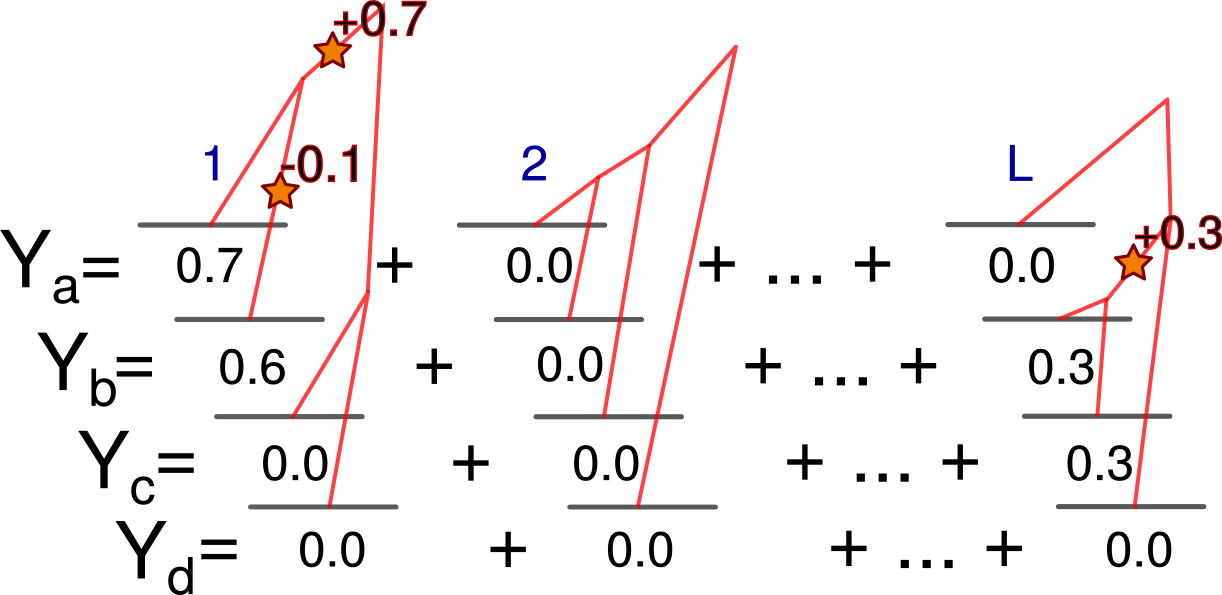
\includegraphics[width=0.9\textwidth]{./figures/schema.png}

  \caption{\textbf{A schematic representation of the model of how we model a
  trait distributions arising from genealogical and mutational distributions.}
  $L$ loci affect the trait in a set of individuals and have independent
  genealogies. Mutations occur within loci as a Poisson process and act
  additively to give individual trait values. Many loci with the potential to
  affect the trait may receive no mutations.}

  \label{fig:schema}
\end{figure}

Here we refer to the genetic parameters of a trait as the combination of
quantities not influenced by the genealogical process: ($L$, $\T$, $\psi$).
Another quantity useful for describing a trait's distribution is its sparsity.
Sparsity should reflect how many mutations segregating in the population
influence the trait, with a more `sparse' trait being one affected by fewer
segregating mutations. Formally, we measure sparsity as the average number of
pairwise differences between two randomly chosen haplotypes at loci affecting
the trait. A trait with fewer causal pairwise differences is more sparse.
Sparsity thus depends both on the genetic parameters through the mutation rate,
the number of potentially causal loci, and the distribution of coalescence
times.

In populations of exchangeable individuals, a useful way to summarize the
distribution of genealogies is through the moments of $\mathbbm{T}_{k,n}$ which
denotes the amount of time that $k$ lineages remain in the genealogy of a sample
of size $n$. The pairwise coalescent time between a lineage in individual $i$
and in individual $j$ is written as $\mathcal{T}_{i,j}$. When considering
structured populations, $\mathcal{T}_{a,b}$ is also used to denote the
coalescence time between a randomly chosen lineage from subpopulation $a$ and a
randomly chosen lineage from subpopulation $b$. A final set of quantities are
defined for sums of branch lengths. Let $\tau_{a+b}$ be the sum of all branches
ancestral to both $a$ and $b$, and $\tau_{a/b}$ be the sum of all branches
ancestral to $a$ but not $b$. Extensions of this for more than two individuals
are also used. The same notation is used when referring to sets of branch
indices. So $\Omega_{a+b}$ and $\Omega_{a/b}$ would be the sets of branches
added to get $\tau_{a+b}$ and $\tau_{a/b}$ respectively.

%%% Local Variables:
%%% TeX-master: "short_report.tex"
%%% End:

\section{The moment generating function for the distribution of trait values}
We first derive the mgf of the distribution of trait values following closely
the approach of \citet{Schraiber2015} and \citet{Khaitovich2005}, but
generalizing to arbitrary demographies and population structure. We consider the
distribution of trait values over evolutionary realizations of the combined
random processes of drift and mutation. The probability distribution for a trait
is complex in its general form. There is a point mass at zero corresponding the
possibility that no mutations occur, and mutational effects could be drawn from
discrete or continuous distributions. Correlations between individuals arise
because of shared history in genealogies at individual loci. Deriving the
cumulative distribution function for trait values may be possible in some
instances, but the difficulty of integrating over mutational configurations
makes it practically impossible for most cases.

However, we can use the mgf approach to study the distribution of trait values.
Following the definition of the mgf for a vector-valued random
variable \citep{Ross}, the mgf for a trait controlled by a single nonrecombining
locus is
\begin{equation}
  \label{eq:mgfdef}
  \varphi_{\mathbf{Y}}(\mathbf{k}) = \E\left[ e^{\mathbf{k} \cdot \mathbf{y}} \right] =
  \int e^{\mathbf{k} \cdot \mathbf{Y}} \Pro(\mathbf{Y}=\mathbf{y}) \mbox{d}\mathbf{y}.
\end{equation}
The vector $\mathbf{k}$ contains dummy variables for each individual, and the
whole operation is an intergral transform of the probability distribution of
trait values. Equation \eqref{eq:mgfdef} can be rewritten by conditioning on the
genealogy to give
\begin{align}
  \label{eq:cond}
  \varphi_{\mathbf{Y}}(\mathbf{k}) &= \int_{\mathbf{Y}} e^{\mathbf{k} \cdot \mathbf{y}}
  \int_{\mathbf{T}} \Pro(\mathbf{Y}=\mathbf{y} | \mathbf{T}=\mathbf{t}) \Pro(\mathbf{T}=\mathbf{t})
  \mbox{d}\mathbf{t} \mbox{d}\mathbf{y} \nonumber \\
  &= \int \int e^{\mathbf{k} \cdot \mathbf{y}} \Pro(\mathbf{Y}=\mathbf{y} | \mathbf{T}=\mathbf{t}) \mbox{d}\mathbf{y}
  \Pro(\mathbf{T}=\mathbf{t})
  \mbox{d}\mathbf{t}.
\end{align}

To proceed, assumptions about the mutational process must be made. The first is
that mutations occur as a Poisson process along branches and the second is that
mutations at a locus are additive. The changes in the trait value along each
branch are then conditionally independent given the branch
lengths. \citet{Khaitovich2005} and \citet{Schraiber2015} noted that this
describes a compound Poisson process. The mgf of a compound Poisson process with
rate $\lambda$ over time $t$ is $\exp(\lambda t (\psi(k)-1))$, where $\psi$ is
the mgf of the distribution of jump sizes caused by events in the Poisson
process \citep{kingman-poisson-processes}. Here, jump sizes are the effects on
the trait value caused by new mutations. Using the mgf of a compound Poisson
process, along with the fact that the mgf of the joint distribution of two
perfectly correlated random variables with the same marginal distribution is
$\varphi_{X_1,X_2}(k_1,k_2)=\varphi_{X_1}(k_1+k_2)$, we can rewrite
equation \eqref{eq:cond} as
\begin{equation}
  \label{eq:fullmgf}
  \varphi_{\mathbf{Y}}(\mathbf{k}) = 
  \int \prod_{\omega \in \Omega} \exp\left( \frac{\theta}{2} t_{\omega} \left( \psi\left(\sum_{a \in \omega}k_{a}\right) -1 \right)\right)
  \Pro(\mathbf{T}=\mathbf{t})\mbox{d}\mathbf{t}.
\end{equation}
Equation \eqref{eq:fullmgf} is the mgf of $\mathbf{T}$ with the dummy variable
$s_{\omega}$ for branch $T_\omega$ set to
$\frac{\theta}{2} \left( \psi(\sum_{a \in \omega}k_{a}) -1 \right)$. This
implies that
\begin{equation}
  \label{eq:sub}
  \varphi_{\mathbf{T}}(\mathbf{s})\Bigr|_{s_{\omega}=\frac{\theta}{2} \left( \psi\left(\sum_{a \in \omega}k_{a}\right) -1 \right)}.
\end{equation}

Thus, if the mgf of the distribution of branch lengths is known, equation
\eqref{eq:fullmgf} allows us to obtain the mgf of the trait values through a
substitution. When the trait is controlled by $L$ independent loci, the full mgf
is obtained by raising equation \eqref{eq:sub} to the power $L$. This result
obviates the need for separate derivations for particular models of population
history and structure.
\citet{Lohse2011} derived the mgf of the genealogy in various population models
including migration and splitting of subpopulations. Using their result for a
single population we can obtain equation (1) of \citet{Schraiber2015} using
equation \eqref{eq:sub} and equation (5) of \citet{Lohse2011}
(Appendix \ref{slrederive}). 

%%% Local Variables:
%%% TeX-master: "quant_gen_manu.tex"
%%% End:

\section{The infinitesimal limit}
This general model converges to a normal model when the infinitesimal limit is
taken. This can be done by first substituting Taylor series for the genealogical
and mutational distributions in equation \eqref{eq:fullmgf}. The infinitesimal
limit should correspond to the situation where the effect sizes of mutations
becomes small as the number of loci becomes large. Assuming mutation rates are
low such that at most one mutation occurs per locus, the resulting distribution
is multivariate normal where the expected trait value is $E[T_{MRCA}] \mu$, the
variance is $E[T_{MRCA}]\sigma^2$, and the covariance between trait values in
two individuals $a$ and $b$ is $E[\tau_{a+b}] \sigma^2$. This limit requires
that the products of $L$ and moments three and greater of the mutational
distribution go to zero as the number of loci becomes large and the effect size
per mutation becomes small. This can be thought of as requiring the mutational
distribution to not have too fat of tails. Details of the derivation and a
generalization to allow multiple mutations per locus are given in
Appendix \ref{clt}.

In this normal distribution, $\mu$ can be interpreted as the rate of change in
the mean trait value per generation per genome due to mutational pressure.
$\sigma^2$ can be interpreted as the rate of accumulation of variance in trait
values per generation per genome. Interestingly, the rate of variance
accumulation is proportional to the second moment of the mutational distribution
and not to the variance. The intuition for why this is can be seen by
considering a degenerate distribution where each mutation has the same effect.
In such a case we would still expect variation among individuals because of
differences in the number of mutations they receive even though the variance of
the mutational distribution is zero. The overall variance among individual trait
values thus has a component due to differences in the number of mutations in
addition to a component due to differences in the effects of these mutations.
The first is proportional to the square of the mean mutational effect, while the
second is proportional to the mutational variance, so their sum is proportional
to $m_2$, the mean squared effect. 

Since the trait values are normally distributed, any linear combination of
sampled trait values will be as well. This includes the distributions of
observable quantities like the differences in trait values from some reference
individual or from a sample mean. The distribution of trait differences between
individuals is multivariate normal with mean zero and the following covariance,
\begin{equation}
\Cov[Y_1-Y_2,Y_3-Y_4] = \sigma^2\left( \E[\mathcal{T}_{1,4}] + \E[\mathcal{T}_{2,3}] -
\E[\mathcal{T}_{1,3}] - \E[\mathcal{T}_{2,4}] \right).
\end{equation}
This holds regardless of whether one assumes the per locus mutation rate is low
(Appendix \ref{clt}). The normal model in the infinitesimal limit provides
additional theoretical justification for studies using normal models to look for
differences in selection on quantitative traits between populations
\citep{Ovaskainen2011,Praebel2013,Robinson2015}. Additionally, this implies 
a covariance matrix based on mean coalescent times rather than population split
times should be used when modeling traits as normally distributed in
phylogenetics.

% If we let $L m_1 \to \mu$,
% $L m_2\to \sigma^2$, $L m_i\to 0$ for $i>2$, and $L^i\left(\T\right)^j \to
% 0$ for $i<j$ as $L\to \infty$, this yields
% \begin{equation}
%   \label{eq:clt}
%   \exp \left( \sum_{\omega \in \Omega}\E[T_{\omega}] \left( \mu \left(
%   \sum_{a \in \omega} k_a\right) + \frac{\sigma^2}{2}\left( \sum_{a \in \omega}
%   k_a\right)^2\right)\right).
% \end{equation}

%%% Local Variables:
%%% TeX-master: "short_report.tex"
%%% End:
 

\section{Low-mutation-rate approximation} \label{sec:lmr}
Thus far, the model assumes that loci are unlinked and can experience an
infinite number of mutations. However, a useful simplification is to ignore the
possibility of more than one mutation per locus. This approximation is
reasonable as long as the nucleotide positions affecting the trait are loosely
linked throughout the genome. The low-mutation-rate approximation greatly
simplifies the mgf of the trait distribution such that it is no longer necessary
to know the full form of the mgf of the genealogy:
\begin{equation}
\label{eq:lowmut}
\varphi_{\mathbf{Y}}(\mathbf{k}) \approx \left[ 1 + \sum_{\omega \in \Omega}
  \E[T_\omega] \T \left( \psi\left( \sum_{a \in \omega} k_a\right) -1 \right) +
  O\left( \theta^2 \right))\right]^L.
\end{equation}
Equation \eqref{eq:lowmut} ignores terms that are order two and above in the
mutation rate. Conveniently this equation depends only on the expected length of
each branch, whereas equation \eqref{eq:fullmgf} requires second order and
greater moments of branch lengths (e.g. $\E[T_{\omega_1}T_{\omega_2}]$). We can
use equation \eqref{eq:lowmut} to express moments of the trait distribution in
terms of expected branch lengths calculated from coalescent models.

%%% Local Variables:
%%% TeX-master: "short_report.tex"
%%% End:

\section{Moments of the trait distribution}
\newcommand{\AAA}{\E[\mathbbm{T}_{4,4}] + \frac{1}{3}\E[\mathbbm{T}_{3,4}] + \frac{2}{9}\E[\mathbbm{T}_{2,4}]}
\newcommand{\BBB}{\frac{1}{9}\E[\mathbbm{T}_{2,4}] + \frac{1}{6}\E[\mathbbm{T}_{3,4}]}
\newcommand{\CCC}{\E[\mathbbm{T}_{4,4}] - \frac{1}{6}\E[\mathbbm{T}_{3,4}] - \frac{1}{9}\E[\mathbbm{T}_{2,4}]}

For most population genetic models and reasonable sample sizes, the recursive
nature of the trait distribution mgf makes it computationally unfeasible to
solve under general parameter values. However, it is not necessary to have an
expression for the full mgf in order to derive moments of the trait distribution
in terms of moments of branch lengths and mutational effects. Under the low
mutation rate approximation moments can be calculated by differentiating
equation \eqref{eq:lowmut}. Even without making this approximation, moments can
be calculated by taking Taylor expansions in equation \eqref{eq:cond} and only
considering terms contributing to the desired moment's order. We implemented a
symbolic math program to calculate trait moments using this procedure, and the
details are given in Appendix ~\ref{symmath}. As the normal distribution is
completely defined by its first two moments, the extent to which a trait
distribution deviates from normality can be measured by the extent to which its
moments deviate from those of a normal distribution with the same mean and
variance.

We have so far considered the distribution of a trait value $Y_a$ over
evolutionary realizations. The expectation of $Y_a$ is $L \T m_1 \E[T_{MRCA}]$,
and the variance is $L \T m_1 \E[T_{MRCA}] + L(m_1^2\T)\Var[T_{MRCA}]$. Although
simple to derive using computer algebra, expressions for the higher central
moments of $Y_a$ are complicated even under the low mutation rate approximation,
and there is not much to be gained by showing them here.

However, in a given evolutionary realization there will be a distribution of
trait values in the population. The population-level trait distribution can also
be described by its moments, but unlike the moments of $Y_a$ the moments at the
population level are random quantities. Since $Y_a$ is relative to a value that
is not directly observed, we can gain more insight by considering the expected
population-level moments. In particular, we are interested in how trait
distribution at the population level might deviate from normality.
~\citet{Schraiber2015} computed the expected first four central moments of a
constant-size population. We derived the same expectations under an arbitrary
demographic history,
\begin{subequations} \label{eq:emoms}
\begin{align}
  &\E[M_2] = L \T \E[\mathbbm{T}_{2,2}] m_2 \label{eq:emoms2}\\
  &\E[M_3] = L \T \E[\mathbbm{T}_{3,3}] m_3  \label{eq:emoms3}\\
  &\E[M_4] = 3\left(L \T \E[\mathbbm{T}_{2,2}] m_2\right)^2 \nonumber \\
  &+ 3\L \left(\T m_2\right)^2\Var[\mathbbm{T}_{2,2}] + \frac{1}{3}
  L \left(\T m_2\right)^2
    \left( \frac{11}{9} \E[\mathbbm{T}_{2,4}^2]-\frac{1}{3}\E[\mathbbm{T}_{2,4}\mathbbm{T}_{3,4}]-
    \frac{1}{4}\E[\mathbbm{T}_{3,4}^2]\right) \nonumber \\
  &+ L m_4 \T ( \E[\mathbbm{T}_{4,4}] + \frac{1}{3} \E[\mathbbm{T}_{3,4}] +
    \frac{2}{9} \E[\mathbbm{T}_{2,4}] ).
  \label{eq:emoms4}
\end{align}
\end{subequations}
To give insight into how the expression in equation \eqref{eq:emoms}, moment
calculations done by hand under the low mutation rate approximation are
presented in Appendix \ref{moments}.

Equation \eqref{eq:emoms2} gives the expected trait variance in the population.
However, the amount of variance will vary over realizations of the evolutionary
process. The variation in the population variance depends on the sparsity of the
trait and the number of causal loci. A certain expected variance can arise
either by multiple mutations at one locus or by multiple mutations each at a
different, independent locus. The variation in the variance can be quantified
using the coefficient of variation of the variance (CVV), the standard deviation
of the variance divided by its expectation. For a constant-size, panmictic
population
\begin{equation}
  \label{eq:cvv}
  \mathrm{CVV} = \sqrt{\frac{4}{3}\frac{1}{L} +
    \frac{1}{6}\frac{\kappa}{L\theta \E[\mathbbm{T}_{2,2}]}}.
\end{equation}
Equation \eqref{eq:cvv} shows a contribution due to linkage that decreases like
$1/\sqrt{L}$ and a contribution due to sparsity that decreases like
$1/\sqrt{L\theta \E[\mathbbm{T}_{2,2}]}$. Even when the sparsity is low, if the
trait is only controlled by a single locus there will be considerable variation
in the population variance (CVV$=\sqrt{\frac{4}{3}}$). On the other hand, the
CVV of a sparse trait controlled by many loci will depend on the mutational
kurtosis as well.
%%% Local Variables:
%%% TeX-master: "short_report.tex"
%%% End:

\section{Comparison to normal distribution}
Deviations of the wihtin-population distribution from normality depend on the
distribution of coalescent times and the genetic parameters. One natural way to
quantify a distribution's deviation from normality is using its kurtosis. The
kurtosis, defined as $M_4/M_2^2$, measures the tendency of a distribution to
produce outliers \citep{Westfall2014}. However, since the kurtosis is a ratio of
two random variables, its expectation is challenging to calculate. Rather than
attempt this calculation, we compare the expected fourth central moment itself
to that expected under normality. This approach qualitatively identifies the
factors influencing deviations from normality.

Using the low mutation rate approximation, the ratio of the expected fourth
moment to that under normality simplifies to
\begin{equation}
  \label{eq:popmom4coal}
  \frac{\E[M_4]}{3\left(L \T \E[\mathbbm{T}_{2,2}] m_2\right)^2} \approx 1 +
  \underbrace{\frac{m_4}{m_2^2}}_{\text{mutation}} \underbrace{(6 L \T \E[\mathbbm{T}_{2,2}])^{-1}}_{\text{sparsity}}
      \underbrace{\left( \frac{2\E[\mathbbm{T}_{4,4}] +
      \frac{2}{3}\E[\mathbbm{T}_{3,4}] +
      \frac{4}{9}\E[\mathbbm{T}_{2,4}]}{\E[\mathbbm{T}_{2,2}]}\right)}_{\text{demography}}
\end{equation}
The expected excess in $M_4$, relative to normality, increases with sparsity and
with $m_4/m_2^2$. $m_4/m_2^2$ is equal to the kurtosis of the mutational effect
distribution when mutations are unbiased and reflects its propensity to produce
large effect mutations. The excess depends on demography through the factor $Q
= \frac{2\E[\mathbbm{T}_{4,4}] + \frac{2}{3}\E[\mathbbm{T}_{3,4}]
+ \frac{4}{9}\E[\mathbbm{T}_{2,4}]}{\E[\mathbbm{T}_{2,2}]}$. The extent to which
demography increases or decreases deviations from normality can be investigated
by calculating $Q$ in different models. In a constant-size, panmictic population
$Q$ is one. In unstructured population, $\E[\mathbbm{T}_{k,n}]$ can be
calculated numerically using expressions from \citet{Griffiths1998}
or \citet{Polanski2003a}. Values of $Q$ in an exponentially growing population
are shown in Figure \ref{fig:Qexp}A. Holding sparsity and the mutational
distribution constant, a population which underwent exponential growth will have
a greater expected deviation from normality in its trait distribution. Another
example demography is a population that goes through a step change at some point
in the past. Figure \ref{fig:Qexp}B shows that when the population size
increased at some point in the past, $Q$ is increased similarly to the
exponential growth scenario. When the population experiences a bottleneck, $Q$
is decreased below one. $Q$ also appears more sensitive to population growth
than to bottlenecks.

\begin{figure}
\centering
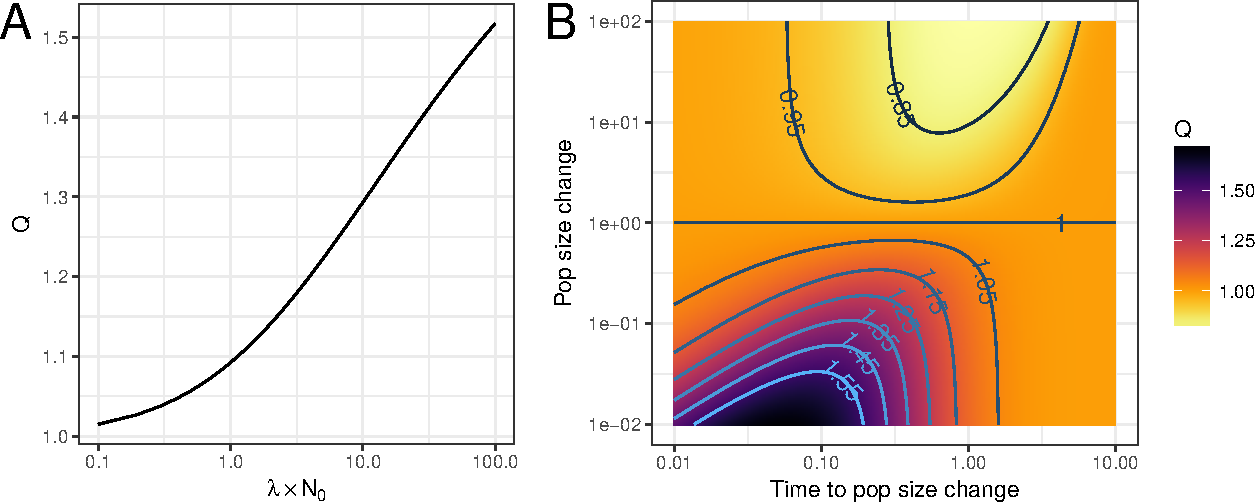
\includegraphics[width=\textwidth]{./figures/combo_q.pdf}
\caption{
\textbf{The effects of demography on deviations of the expected
fourth central moment of the population trait distribution from normality.} $Q$
measures the effect due to demography on the expected fourth central moment
(equation \eqref{eq:popmom4coal}). (\textbf{A}): $Q$ increases as the
exponential growth rate increases relative to the current population
size.~$\lambda$ is the growth rate and $N_0$ is the initial effective population
size.~(\textbf{B}): $Q$ values when the population undergoes an instantaneous
step change at some point in the past. The time and magnitude of this change are
given in units of the current effective population size. $Q$ increases when the
population grows and decreases when it declines.}
\label{fig:Qexp}
\end{figure}

\begin{figure}
\centering
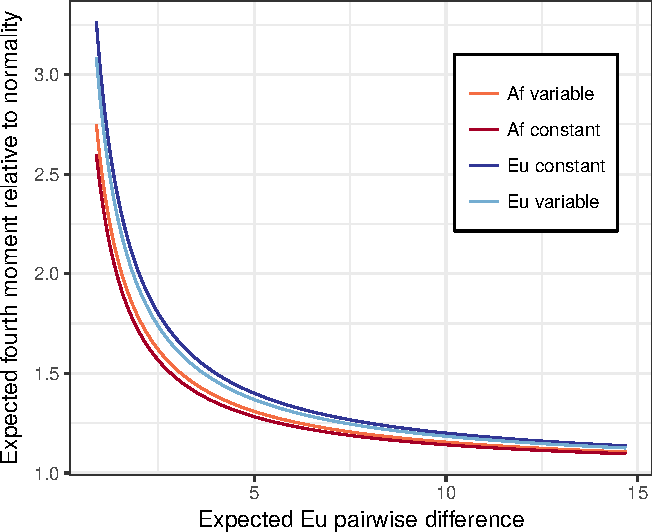
\includegraphics[width=0.55\textwidth]{./figures/af_eu_mom4_r.pdf}
\caption{ \textbf{A comparison between the expected fourth moment at different levels of
sparsity in the African and European demographic models fit
by \citet{Tennessen2012}.} Trait sparsity is varied by changing the expected
number pairwise differences at sites affecting the trait in the European model.
The mutational kurtosis is set to six. The darker lines show the predicted
relationship for populations with the same heterozygosity as the European and
African models but with constant size.}
\label{fig:afeucomp}
\end{figure}

As a concrete example, we can consider the differences in the expected fourth
moment produced by demographic histories in different human populations. In the
demographic model fit by \citet{Tennessen2012}, the generic European population
experiences an out-of-Africa bottleneck followed by recent growth, while the
generic African population experiences a more stable history also with recent
growth. Differences in demographic history between the two populations has
resulted in a lower heterozygosity in European populations due to the
out-of-Africa bottleneck \citep{Yu2002}.

For a given sparsity, the African population model predicts a smaller deviation
from normality than the European model (Figure \ref{fig:afeucomp}). The expected
fourth moment in constant-size populations with the same heterozygosity as the
African and European models is lower for the African model and higher for the
European model. This is because the African model is dominated by population
growth that leads to a $Q$ greater than one, while the European model is
dominated by a bottleneck event that leads to a $Q$ less than one (Figure
\ref{fig:Qexp}). However, differences due to demography are small and deviations
from normality are mostly driven by differences in sparsity.

Even though recombination is not modeled, we can speculate on how linkage
impacts deviations from normality. Line two of equation \eqref{eq:emoms4}
corresponds to the contribution from two mutations occurring at a single locus.
The first quantity indicates that the expectation of the fourth moment increases
with the variance of the pairwise coalescence time. The second part does not
have a clear interpretation. If the sum of these two terms is positive this
agrees with the intuition that linkage disequilibrium increases deviations from
normality by reducing the effective number of independent loci.

Simulations of the kurtosis itself show substantial variance, with about a
quarter of simulated populations having a value less than three (that of a
normal distribution) even as the mean kurtosis increases to almost nine
(Appendix \ref{kurtsim}). This high variance in the kurtosis is likely due to a
high variance in both the variance and fourth moment. This, along with the fact
that deviations from the infinitesimal model inflate the fourth moment
(equation \eqref{eq:popmom4coal}), leads to a situation where the kurtosis
increases with trait sparsity but the variance is high across evolutionary
realizations.
%%% Local Variables:
%%% TeX-master: "quant_gen_manu.tex"
%%% End:

\section{Trait divergence in structured populations}
\begin{figure}
  \centering
  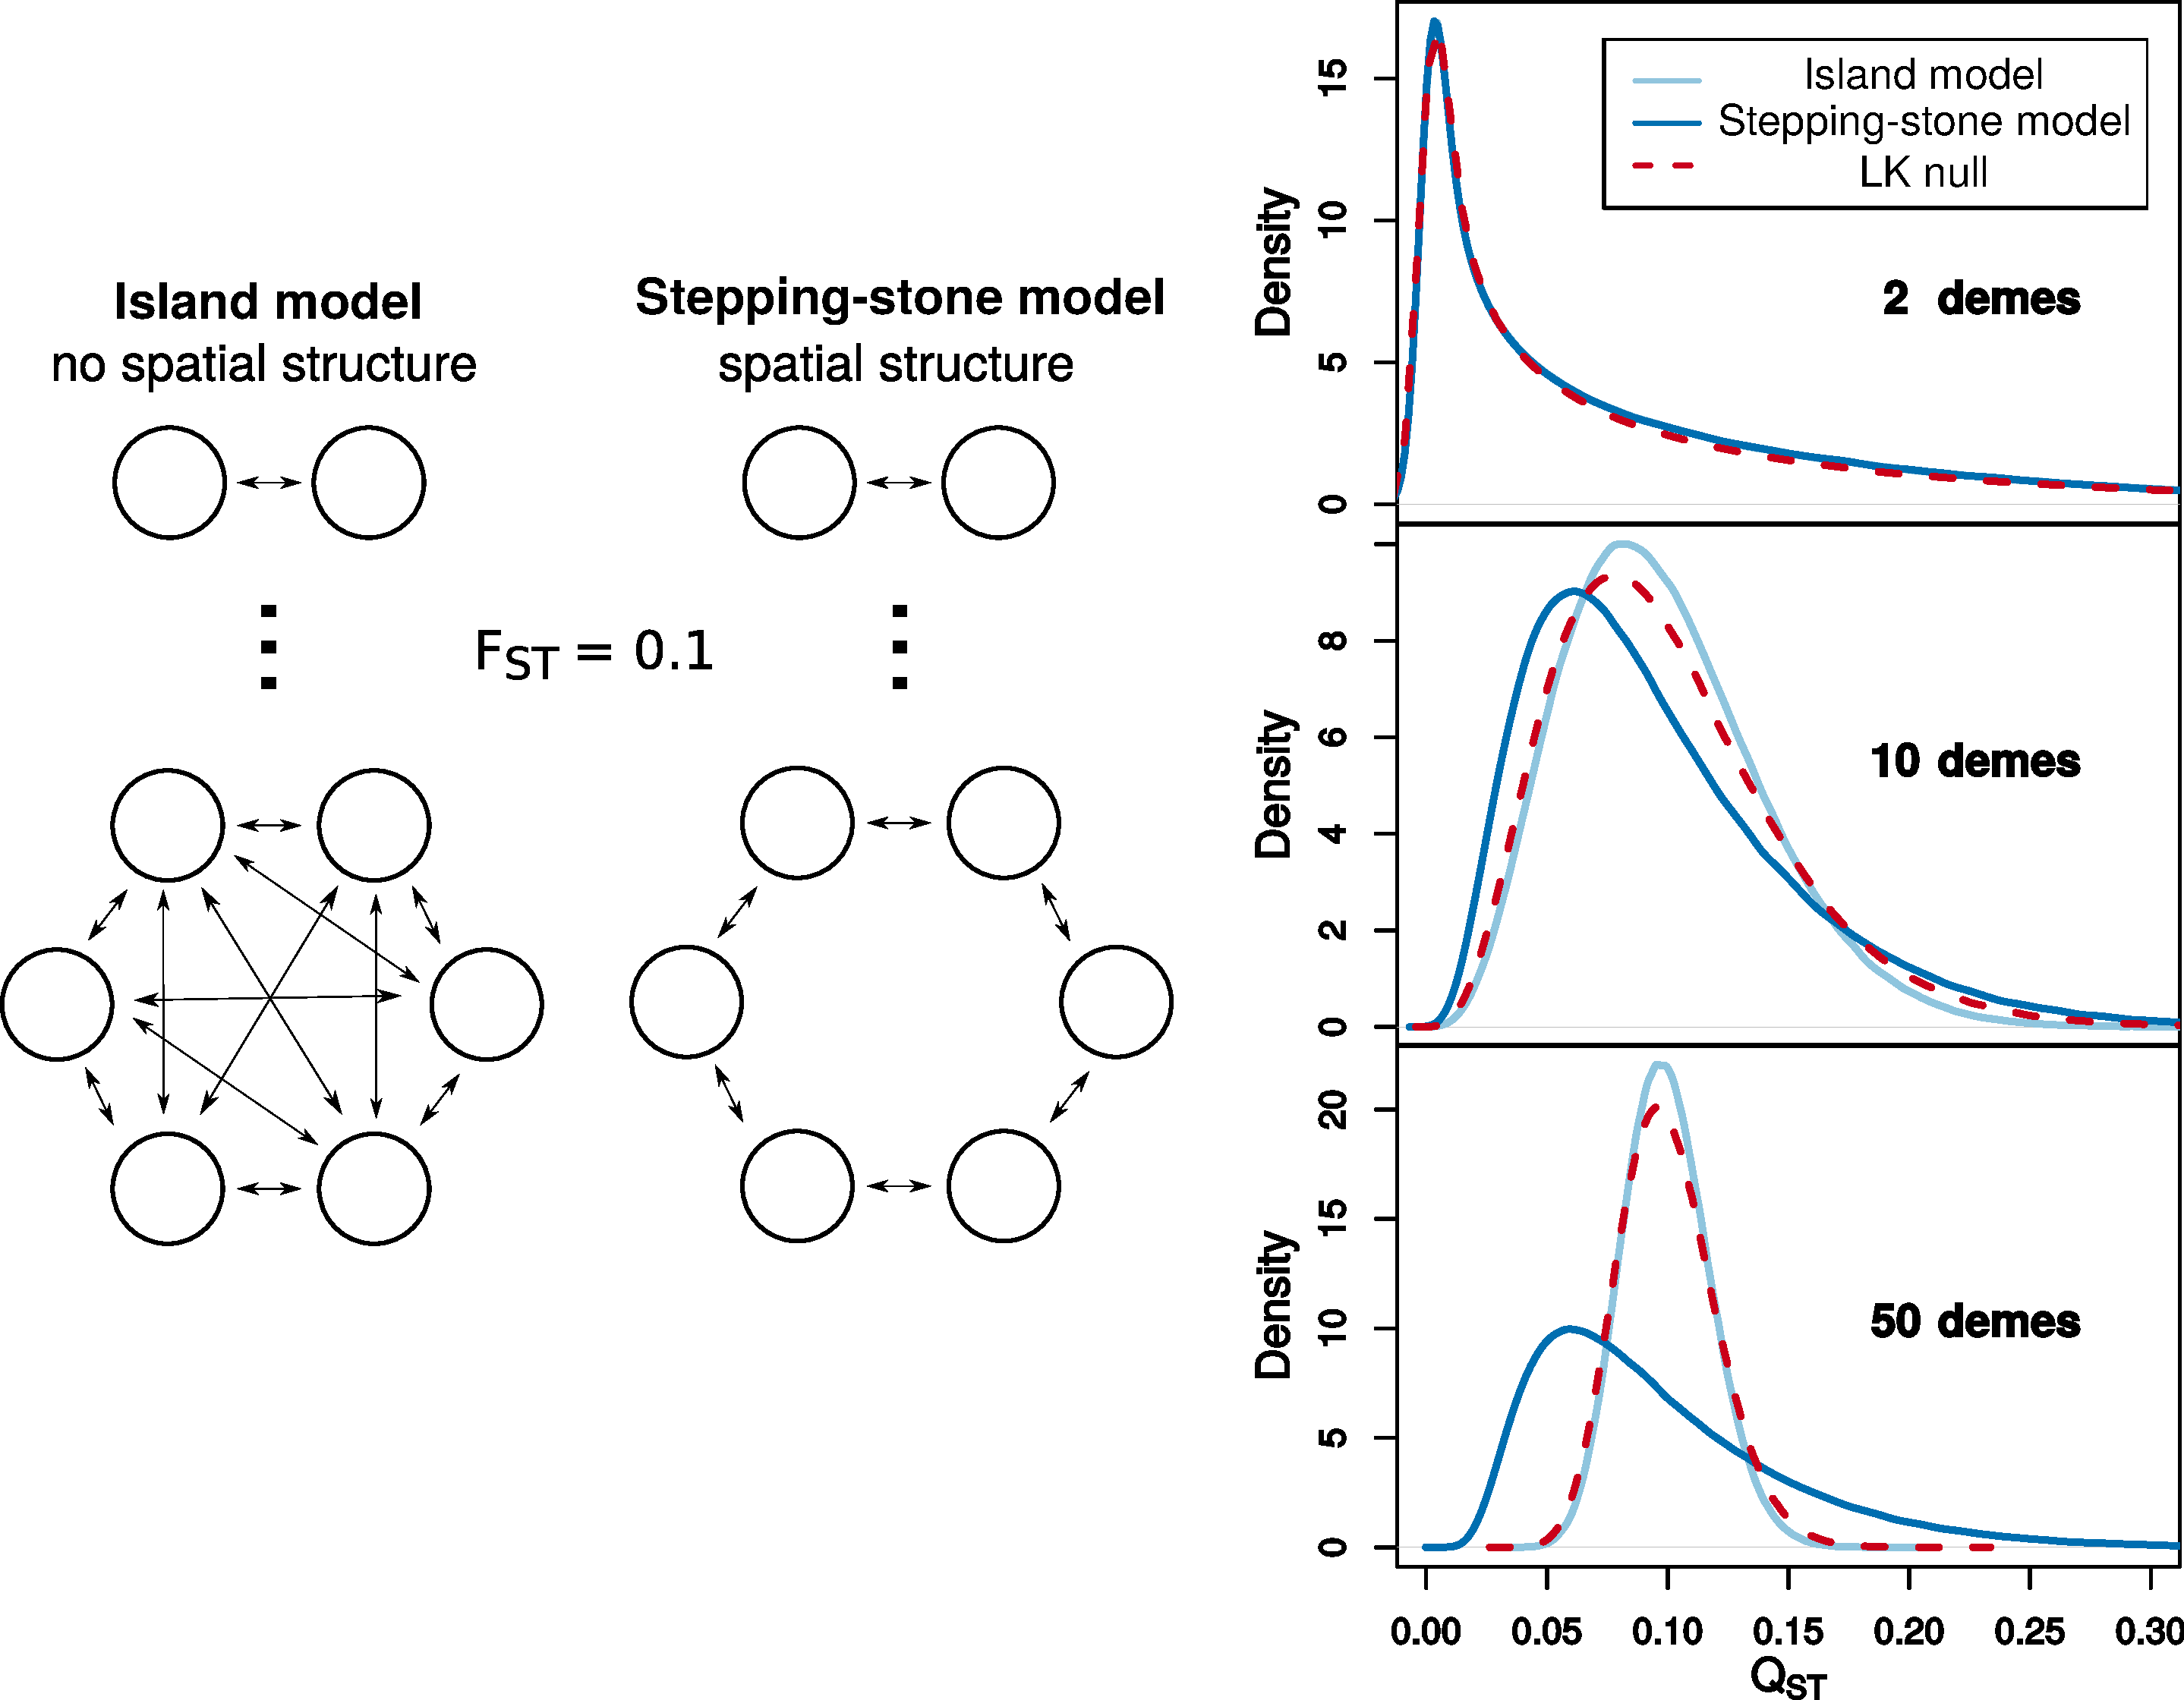
\includegraphics[width=0.95\textwidth]{./figures/pop_struct_combine_alt.pdf}
  \caption{ \textbf{A comparison of neutral sampling distributions for $Q_{ST}$
      at the population level.} The Lewontin-Krakauer (LK) distribution for
    $Q_{ST}$ is compared to the null distribution in the infinitesimal limit in
    a case with (the stepping-stone model) and a case without (the island model)
    spatial structure. The case with no spatial structure assumes the migration
    rate is equal between all subpopulations, and the case with spatial
    structure arranges subpopulations in a ring with migration only between
    neighboring subpopulations. Migration rates and subpopulation sizes are all
    equal and are set such that $F_{ST}=0.1$ even as the number of
    subpopulations is increased \citep{Slatkin1991}. $Q_{ST}$ values for these
    models are simulated by drawing vectors from a multivariate normal
    distribution parameterized using the expected pairwise coalescence times
    given by \citep{Slatkin1991}. Under the LK distribution $Q_{ST}$ is
    distributed as $F_{ST}/(n_d - 1)$ times a chi-square distribution with $n_d
    - 1$ degrees of freedom ($Q_{ST}\sim F_{ST}\chi^2_{n_d - 1}/(n_d-1)$), where
    $n_d$ is the number of subpopulations. Vertical lines show the mean $Q_{ST}$
    under the different null distributions. The mean $Q_{ST}$ values for the two
    normal models are nearly identical. Discordance between these lines and that
    for the LK distribution illustrates that $Q_{ST} \neq F_{ST}$. The neutral
    distributions for $Q_{ST}$ become increasingly different as the number of
    subpopulations over which the genetic divergence is spread increases.}
  \label{fig:qst_deme}
\end{figure}

\begin{figure}
  \centering
  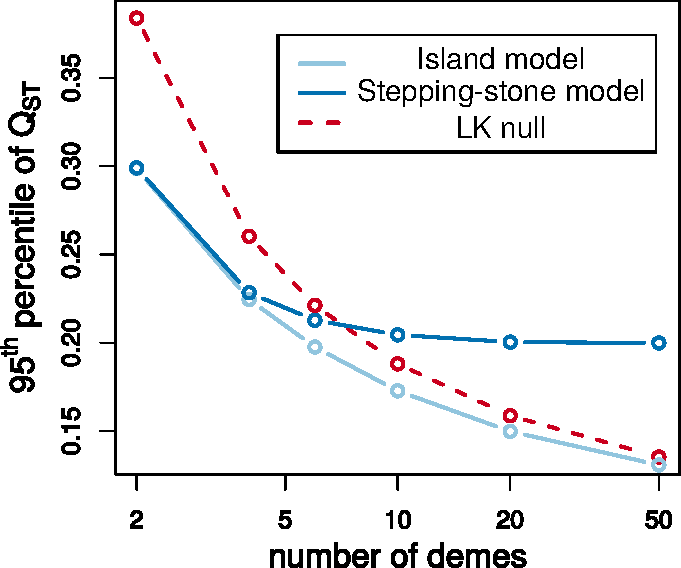
\includegraphics[width=0.5\textwidth]{./figures/qst_deme_percentile_nospace_alt.pdf}
  \caption{\textbf{Differences in the $95^{\mathrm{th}}$ percentile of different
      neutral sampling distributions for $Q_{ST}$ at the population level.} The
    Lewontin-Krakauer (LK) distribution is compared to neutral null
    distributions for structured populations with and without a spatial
    component using the multivariate normal model that arises in the
    infinitesimal limit.}
  \label{fig:qst_perc}
\end{figure}


To demonstrate the utility of the normal distribution arising in the
infinitesimal limit (equation \ref{eq:normcov}), we derive a simple procedure
for simulating from null distribution for the divergence between groups in
structured populations. A common way to quantify the divergence in trait values
between groups is $Q_{ST}$, defined as the variance between the group means
divided by the total variance in the population \citep{Spitze1993}. In a haploid
model, $Q_{ST} = \frac{V_{between}}{V_{between} + V_{within}}$, where
\begin{equation*}
  V_{between} = \frac{1}{K} \sum_i \left( \bar{Y}_i - \bar{Y} \right)^2
\end{equation*}
and
\begin{equation*}
  V_{within} = \frac{1}{\sum_k N_k} \sum_i \sum_j \left( Y_{i,j} - \bar{Y}_i \right)^2.
\end{equation*}
Here, $Y_{i,j}$ is the trait value of individual $j$ in population $i$, $K$ is
the number of subpopulations, and $N_k$ is the size of subpopulation $k$.

In the normal model, all $Y_{i,j}$ are normally distributed. Therefore,
$\bar{Y}_{i} - \bar{Y}$ and $Y_{i,j} - \bar{Y}_i$ are also normally distributed.
When population sizes are large, individual deviations from population means are
nearly uncorrelated, as are $V_{between}$ and $V_{within}$. $V_{within}$ is
nearly constant across evolutionary realizations and is equal to $\sum_k N_k
E[\mathcal{T}_{k,k}] / \sum_k N_k$ because the within population variances are
approximately uncorrelated and their variances are order $1/N_k$. While we do
not have an explicit form for the density function of the between-group
variance, we can simulate from its distribution by drawing a vector of
$\bar{Y}_{i} - \bar{Y}$ values from a multivariate normal distribution with mean
zero and with a covariance matrix whose element between populations $a$ and $b$
is
\begin{equation}
  \Cov[\bar{Y}_{a} - \bar{Y}, \bar{Y}_{b} - \bar{Y}] =
  \mu_2 \T (\E[\mathcal{T}_{a,\cdot}] + \E[\mathcal{T}_{b,\cdot}] -
  \E[\mathcal{T}_{\cdot,\cdot}] - \E[\mathcal{T}_{a,b}]).
\end{equation}
To simulate $Q_{ST}$ values we do not need to know $\mu_2$ or $\T$ because the
scale of the trait variance cancels in the $Q_{ST}$ ratio. Therefore, all that
is necessary to simulate from the null distribution of $Q_{ST}$ is to have
estimates of the expected coalescent time within and between populations. No
further information about the history or structure of the population is needed.
Since only the relative coalescent times matter it is also not necessary to
scale these estimates to units of years or generations using a mutation rate.

This procedure for simulating from the null distribution of $Q_{ST}$ could be
useful in testing whether an observed $Q_{ST}$ is unlikely under neutrality.
Current goodness-of-fit tests either compare $Q_{ST}$ to an empirical
distribution of $F_{ST}$ values or to a $\chi^2$ distribution
\citep{Leinonen2013}. In the second case, an identical distribution to that
developed by \citet{Lewontin1973} is used as the null distribution for $Q_{ST}$.
The $\chi^2$ testing procedure was suggested by \citet{Whitlock2009} and is
implemented in the program \textit{QstFstComp} \citep{Gilbert2015}. The
Lewontin-Krakauer (LK) distribution assumes independence between subpopulations
and provides a good approximation in populations without spatial structure, such
as in a symmetric island model of migration (Figure \ref{fig:qst_deme}). When
subpopulations are strongly correlated, such as in a one-dimensional
stepping-stone model of population structure, the LK distribution is a poor
approximation. Even when the distributions appear qualitatively similar, there
are substantial differences in tail probabilities (Figure \ref{fig:qst_perc}).

Nearly identical issues to these were raised with the LK test at the time of its
publishing \citep{Nei1975,Robertson1975}. However, while the neutral
distribution for $F_{ST}$ depends on the precise details of population structure
and history, the distribution of $Q_{ST}$ only depends on the set of within and
between subpopulation coalescence times. The point here is not that the LK
distribution is particularly bad, but rather that an improved neutral
distribution can be obtained using the normal model arising in the infinitesimal
limit. The neutral distribution described here is similar to the extension of
the LK test developed by \citet{Bonhomme2010} to account for the correlation
structure between subpopulations. The \citet{Bonhomme2010} method treats allele
frequencies as multivariate normal with covariance matrix parameterized by
coancestry coefficients. \citet{Ovaskainen2011} use a normal model similar to
that found in the infinitesimal limit here, but the covariance matrix is also
based on coancestry coefficients. When phenotypic and genetic divergence is
mostly driven by changes in allele frequency, the coalescent and coancestry
based models should be very similar. However, the coalescent model is ultimately
preferable since it is the correct null model at any scale of population
divergence in the infinitesimal limit. When only allele frequency data are
available, a coancestry model is the only option, but it is still better to
model variable levels of shared ancestry between populations than to use a
single value of $F_{ST}$.

Additionally, treating $Q_{ST}$ as a random variable lets us reexamine the
classic result in evolutionary quantitative genetics that $Q_{ST}=F_{ST}$
\citep{Whitlock1999}. $F_{ST}$, in this context, refers to a parameter of the
population. In particular, $F_{ST} = \frac{\bar{t} - \bar{t}_0}{\bar{t}}$, where
$\bar{t}$ is the expected coalescent time for two loci sampled at random from
the entire population and $\bar{t}_0$ is the expected coalescent time for two
loci sampled within a subpopulation \citep{Slatkin1991}. This value is constant
over realizations of the evolutionary process. $Q_{ST}$ can only refer to either
state of the population or to an estimate of this state. As shown above,
$Q_{ST}$, as a state of the population, varies across evolutionary realizations.
Thus, there is no sense in which $Q_{ST}$ can be defined as a constant parameter
in the way that $F_{ST}$ can. The expectation of $V_{between}$ is $\bar{t} -
\bar{t}_0$, and the expectation of $V_{within}$ is $\bar{t}_0$.
$\frac{\E[V_{between}]}{\E[V_{between}] + \E[V_{within}]}$ is equal to $F_{ST}$,
but due to Jensen's inequality, the expectation of this ratio ($\E[Q_{ST}]$) is
always less than $F_{ST}$.

%%% Local Variables:
%%% TeX-master: "quant_gen_manu.tex"
%%% End:

%% \section{The response to selection}
%% A situation in which higher order moments of the trait distribution can be
relevant is in the response of the population to selection. Evolutionary
quantitative genetics often assumes the distribution of additive genetic values
in the population remains normally distributed as selection alters the mean and
variance. \citet{Turelli1990} used a multilocus population genetic model to show
how departures from normality affect the response to selection. In their
analysis, departures from normality are due to the build up of linkage
disequilibrium. However, their results are valid regardless of how departures
from normality arise. The \citet{Turelli1990} theory can be used to analyze the
response to selection in the toy situation of a trait that has evolved neutrally
up to the current time and is then subjected to one generation of selection
under a particular fitness function.

According to \citet{Turelli1990}, in the absence of environmental effects the
response of the mean phenotype in the population is
\begin{equation}
  \label{eq:selresp}
  \Delta \bar{Y} = M_2L_1 + M_3L_2 + \gamma_4M^2_2L_3 +
  \left( M_5-4M_3M_2\right)L_4 + \ldots.
\end{equation}
$\gamma_4$ is the excess kurtosis of the trait values in the population above a
normal distribution and the $M_i$ terms are again the $i^{th}$ central moments
of the trait value distribution in the population. The $L_i$ are selection
gradients in terms of the moments of the genetic component of the trait value
distribution and describe the shape of the fitness function on the trait values.
In the absence of environmental effects, the $L_i$ are selection gradients in
terms of the moments of the trait value distribution that we have so far
considered in this study.

Equation \eqref{eq:selresp} shows that whether higher order moments of the trait
distribution contribute to the selection response depends on the shape of the
fitness function through the $L_i$. The excess kurtosis affects the response to
selection linearly with $L_3$, which depends on the third moment of the trait
value distribution.

When selection is cubic ($W(Y) = b_0 + b_3(Y-\bar{Y})^3$), the response to
selection is
\begin{equation}
  \label{eq:cubresp}
  \Delta \bar{Z} = \frac{M_4\beta}{1 + M_3\beta},
\end{equation}
where $\beta=b_3/b_0$. Cubic selection represents an idealized fitness function
to investigate the effects of selection acting on the tails of the population
trait distribution. Equation \eqref{eq:cubresp} is a ratio of random quantities,
so calculating the expected response to selection is not feasible. However, we
conjecture that demographic and mutational process increasing the expected
fourth central moment relative to the third would increase the response to
selection. For instance, a high mutational kurtosis and a low skew would likely
increase the response to cubic selection.

%%% Local Variables:
%%% TeX-master: "short_report.tex"
%%% End:

\section{Inferring genetic parameters}
\citet{Schraiber2015} suggested it might be possible to infer something about
the genetic architecture and distribution of mutational effects for sparse
traits whose distributions deviate from normality. Using the expressions for the
expected moments in equation \eqref{eq:emoms} we could imagine a method of
moments estimator for these quantities. If $\hat{D}_{i,j}$ is an estimator of
$\T \E[\mathbbm{T}_{i,j}]$, the system of equations for the first three central
moments under the low mutation rate approximation is
\begin{align}
\label{eq:genearch}
  &\hat{M}_2 = \hat{D}_{2,2}Lm_2 \nonumber \\
  &\hat{M}_3 = \frac{1}{3}\hat{D}_{3,3}Lm_3 \nonumber \\
  &\hat{M}_4 = 3\hat{M}_2^2 + (\hat{D}_{4,4} + \frac{1}{3} \hat{D}_{3,4} + \frac{2}{9} \hat{D}_{2,4})Lm_4.
\end{align}
From equation \eqref{eq:genearch} we can see that the moments of the trait
distribution only enter through products with the number of loci potentially
affecting the trait. Thus, while we can infer the shape of the mutational
distribution, we cannot discern the number of loci affecting a trait from the
magnitude of mutational effect sizes.

%%% Local Variables:
%%% TeX-master: "short_report.tex"
%%% End:

\section{Discussion}
Neutral models of quantitative trait evolution are important for establishing a
baseline against which to test for selection. \citet{Schraiber2015} recently
analyzed a neutral model of trait evolution that made few assumptions about the
number of loci potentially affecting the trait and the distribution of
mutational effects at these loci. However, they only derived results for
constant-size, panmictic populations. We extend their results to populations
with arbitrary distribution of coalescent times and therefore varying
demographies and population structures. As their key result,
\citet{Schraiber2015} derived the characteristic function of the distribution of
trait values in a sample. In this paper, we instead work with the moment
generating function, but the two approaches are interchangeable as long as the
mgf for the distribution of mutational effects exists (which it will if the
moments of the mutational distribution are all finite). Our main result, given
in equation \eqref{eq:sub}, shows that the generating function obtained
by \citet{Schraiber2015} is a special case of a general procedure whereby the
moment generation function for a trait distribution can be obtained by making a
simple substitution into the moment generating function for a distribution over
genealogies. The moment generating functions for many demographies of interest
and for sample sizes above two are sufficiently complex that solving for them is
impractical \citep{Lohse2011}. However, progress can still be made by using
Taylor expansions to write moments of the trait distribution in terms of moments
of the genealogical and mutational distributions.

This result extends previous work using coalescent theory to investigate neutral
models of quantitative traits \citep{Whitlock1999,Schraiber2015}. Ours is the
most general model yet analyzed. As a natural first step, we show that the
infinitesimal limit suggested by \citet{Fisher1918} leads to a model where
phenotypes are normally distributed as the number of loci becomes large and the
variance of effect sizes becomes small. In the limiting distribution, the
variance of the difference in trait values between two individual is
proportional to the expected pairwise coalescent time between them, and the
covariance between a pair of differences more generally is $\Cov[Y_a - Y_b,Y_c -
Y_d] \propto \E[\mathcal{T}_{a,d}] + \E[\mathcal{T}_{b,c}] -
\E[\mathcal{T}_{a,c}] - \E[\mathcal{T}_{b,d}]$. The resulting covariance matrix
completely specifies the neutral distribution under the infinitesimal model.
This is similar to classic models in evolutionary quantitative genetics
considering the neutral divergence of trait values after population splits
\citep{Lande1976,Lynch1989} but holds regardless of the precise details of
population structure and history. \citet{Schraiber2015} derive essentially the
same distribution using a central limit theorem argument. 

\citet{Mendes2018} point out several problems caused by incomplete
lineage sorting when species split times are used to generate the covariance
matrix in phylogenetic comparative methods. Since the normal model arising in
the infinitesimal limit is explicitly based on the coalescent, it is not subject
to these problems. A matrix based on pairwise coalescence times rather than a
species tree based on population split times takes into account the effects of
all lineages at causal loci, even those that do not follow the species topology.
The covariances specified by equation \eqref{eq:normcov} could also be used to
generate within-species contrasts in a similar manner to the method suggested
by \citet{Felsenstein2002}.

We compared sparse traits to the normal model by calculating how the first four
expected central moments different from those expected under normality. This
showed how demography and genetics separately influence the expected deviation
from normality. For a fixed expected trait sparsity, population growth produces
greater deviations in the fourth central moment while population bottlenecks
produce lower deviations (Figures
\ref{fig:Qexp}). However, for realistic demographic scenarios,
we find that the effects attributable to demography are small (Figure
\ref{fig:afeucomp}). We only analyzed cases where the individuals in the
population were exchangeable, but adding population structure would increase
deviations from normality as drifting trait means between subpopulations will
yield a multimodal distribution.

We next apply the above theory to two simple problems where a coalescent
perspective on the neutral distribution of a quantitative trait provides useful
intuition. The first of these is the question of the appropriate null
distribution for $Q_{ST}$ at the population level. We show how the null
distribution under the normal model can be easily simulated from by taking
advantage of the theory presented here, providing a much better approximation
when populations are correlated than previous approaches \citep{Whitlock2009}
(Figure \ref{fig:qst_deme}). In the second we show that the shape of the
mutational distribution is largely confounded with the number of loci affecting
the trait, with only one compound parameter identifiable. This makes it unlikely
that mutational parameters could be inferred from trait values sampled from a
population.

Even though we have broadened the model space for neutral traits, many features
of real populations have not yet been incorporated. Linkage between loci is a
particular concern as there is substantial linkage disequilibrium between QTLs
\citep{Bulik-Sullivan2015}. \citet{Lohse2011} derived the form of the moment
generating function for linked loci and future work will attempt to incorporate
this using equation \eqref{eq:sub}. In particular, it will be important for
future work to show how this affects the distribution in the infinitesimal
limit. Diploidy, dominance, and epistasis have also been ignored thus far. The
qualitative effects described here should hold under diploidy, but having trait
values within individuals summed over loci from two copies of the genome will
decrease deviations from normality. Dominance will also tend to produce a normal
distribution as the effects are independent between loci, but future work is
needed to examine how this interacts with the distribution of genealogies to
affect the trait distribution.

\citet{Barton2017} recently performed a deep mathematical investigation of a
more formal ``infinitesimal model'' that is subtly different from the
infinitesimal limit considered here. They proved conditions under which the
trait values of offspring within a family are normally distributed with variance
independent of the parental trait values conditional on the pedigree and
segregation variance in the base population. Interestingly, they found the
normality for offspring trait values still holds under some forms of pairwise
epistasis that are not too extreme. This implies it may be possible to include
epistasis in the infinitesimal limit considered here. It would be important to
know how epistasis affects the neutral divergence of trait between populations
and species.

Although GWAS of many traits have shown them to be controlled by large numbers
of loci \citep{Boyle2017}, this will not necessarily be the case for every trait
of interest to biologists. It has been suggested, for instance, that gene
expression levels have a sparse genetic architecture \citep{Wheeler2016}. Since
there is much interest in testing whether natural selection has acted on gene
expression levels \citep{Whitehead2006,Gilad2006,Yang2017}, well-calibrated
goodness-of-fit tests will need to take into account the complications that
arise when trait distributions deviate from normality \citep{Khaitovich2005}.
Direct measurements of mutational distributions \citep{Gruber2012,Metzger2016}
could aid in such a calibration. Finally, equation \eqref{eq:emoms} suggests a
means to determine whether sparsity impacts trait distributions by examining
populations with different demographic histories. Populations with a greater
$\mathbbm{T}_{3,3}$ to $\mathbbm{T}_{2,2}$ ratio are also expected to show a
greater $M_3$ to $M_2$ ratio and an equivalent relationship would be expected
for the fourth moment. Because gene expression studies generally measure a large
number of traits, observing such a trend on average could be a sign of
deviations from normality. Generally, more work is needed to develop neutrality
tests that are robust to the details of genetics and population history, and to
investigate whether any information about mutation can be uncovered by
statistical models that share information across multiple measured traits. 

%%% Local Variables:
%%% TeX-master: "quant_gen_manu.tex"
%%% End:

\section*{Acknowledgements}
We thank John Novembre, Daniel Rice, and members of the Novembre lab for helpful
discussions. We would also like to thank Josh Schraiber, Daniel Rice, John
Novembre, Maryn Carlson, Hussein Al-Asadi, and Joe Marcus, as well as two
reviewers for their comments on the manuscript. This work was supported by an
NSF GRFP to the author and NIH grant GM108805 to John Novembre.

\bibliographystyle{genetics} 
\bibliography{quant_gen}
\clearpage

%% APPENDIX %%
\appendix
\beginsupplement

\section{A central limit theorem in the infinitesimal limit}
\label{clt}
The moment generating function for the distribution of trait values from a
single locus is
\begin{equation*}
  \varphi_{\mathbf{Y}}(\mathbf{k}) = \int \exp \left( \sum_{\omega \in \Omega} s_{\omega}t_{\omega} \right)
  \Pro(\mathbf{T}=\mathbf{t})\mathrm{d}\mathbf{t}
  \Bigr|_{s_{\omega}=\frac{\theta}{2} \left( \psi\left(\sum_{a \in \omega}k_{a}\right) -1 \right)}.
\end{equation*}
If we substitute in the Taylor series expansions for the moment generating
function of the trait value distribution we get
\begin{equation*}
  \int \prod_{\Omega} \exp\left[ t_{\omega} \T \left( \sum_{n=1}^{\infty} \frac{m_n}{n!}
    \left( \sum_{a \in \omega} k_a \right)^n \right) \right]
  \Pro(\mathbf{T} = \mathbf{t}) \mathrm{d}\mathbf{t}.
\end{equation*}
If we then write the Taylor series of each exponential function we get
\begin{equation*}
  \int \prod_{\Omega} \left[ \sum_{j=0}^\infty \frac{t_{\omega}^j}{j!}
  \left( \T \right)^j \left( \sum_{n=1}^{\infty} \frac{m_n}{n!}
  \left( \sum_{a \in \omega} k_a \right)^n \right)^j \right]
  \Pro(\mathbf{T} = \mathbf{t}) \mathrm{d}\mathbf{t},
\end{equation*}
which is equivalent to
\begin{equation*}
  1 + \sum_{\Omega} \E[T_\omega] \T \sum_{n=1}^{\infty} \frac{m_n}{n!} \left(
  \sum_{a \in \omega} k_a \right)^n +
  \sum_{\Omega \times \Omega} \frac{1}{2} E[T_{\omega_1}T_{\omega_2}]
  \sum_{n=1}^{\infty} \T \frac{m_n}{n!} \left(\sum_{a \in \omega_1} k_a \right)^n
  \sum_{n=1}^{\infty} \T \frac{m_n}{n!} \left(\sum_{a \in \omega_2} k_a \right)^n + \ldots
\end{equation*}

This is raised to the power $L$ for a trait controlled by $L$ loci. We want the
limit as the number of loci increases while the size of mutational effects
decreases. This can be expressed by the limits $L m_1 \to \mu_1$, $L m_2\to
\mu_2$ and $L m_i\to 0$ for $i>2$ as $L \to \infty$. Knowing we will not be
retaining $m_3$ and above we can rewrite the mgf as
\begin{equation*}
  \left(1 + \sum_{\Omega} \E[T_\omega] \T \left(m_1 \sum_{a \in \omega} k_a +
  \frac{m_2}{2} \left(\sum_{a \in \omega} k_a \right)^2\right)\right)^L.
\end{equation*}
The result of taking these limits is
\begin{equation}
  \label{eq:norm_mgf}
  \exp \left( \sum_{\omega \in \Omega}\E[T_{\omega}] \T \left( \mu_1 
  \sum_{a \in \omega} k_a + \frac{\mu_2}{2}\left( \sum_{a \in \omega}
  k_a\right)^2\right)\right).
\end{equation}

This is multivariate normal distribution with mean equal to $\E[T_{MRCA}] \T \mu_1$,
variance equal to $\E[T_{MRCA}] \T \mu_2$, and covariance between $Y_a$ and $Y_b$
equal to $\E[\tau_{a+b}] \T \mu_2$. This can be seen from equation
\eqref{eq:norm_mgf} by noting that in the mgf for a multivariate normal
distribution the coefficient in the exponential of $k_a$ is the mean of $Y_a$
and the coefficient of $k_ak_b$ is $2\Cov[Y_a,Y_b]$ if $a\neq b$ and $\Var[Y_a]$
if $a=b$.

These $Y$ values are not directly observed because in the theory presented here
they are measured as the sum of differences since the $T_{MRCA}$s at the causal
loci affecting the trait. Rather, differences between individual trait values
are what analyses would be based on. Since the $Y$ are normally distributed
differences between trait values such as $Y_a-Y_b$ will be as well.
\begin{align*}
  \Var[Y_a-Y_b] &= Var[Y_a] + \Var[Y_b] - 2\Cov[Y_a,Y_b]\\
                &= 2(\E[T_{MRCA}] - \E[\tau_{a+b}])\mu_2.
\end{align*}
This also tells us that the distribution of trait differences will be the same
in the infinitesimal limit with and without a low mutation rate approximation.

A much simpler heuristic derivation of the limiting normal distribution can be
done by calculating the variance and covariance at a single locus. This
derivation is very similar to that done by \citet{Schraiber2015}. Using the law
of total variance we can write
\begin{equation*}
  \Var[Y] = \E\left[\Var[Y|T]\right] +
  \Var\left[\E[Y|T]\right]
\end{equation*}
The variance conditional on $T$ can be calculated again using the law of total
variance and conditioning on the number of mutations at the locus. 
\begin{align*}
  \Var[Y|T] &= \E[\Var[Y|M]|T] + \Var[E[Y|M]|T]\\
            &= \E[M(m_2-m_1^2)|T] + \Var[Mm_1|T]\\
            &= \T T (m_2-m_1^2) + \T T m_1^2\\
            &= \T T m_2
\end{align*}
\begin{align*}
  \E[Y|T] = \T T m_1\\
  \Var[\T T m_1] = \left( \T m_1\right)^2\Var[T]
\end{align*}
Therefore we have
\begin{equation}
  \Var[T] = \T m_2 \E[T_{MRCA}] + (\T m_1)^2 \Var[T_{MRCA}].
\end{equation}

The same procedure can be done for the covariance.
\begin{equation*}
  \Cov[Y_a,Y_b] = \E[\Cov[Y_a,Y_b|T]] + \Cov[E[Y_a|T],E[Y_b|T]]
\end{equation*}
We can break $Y_a$ and $Y_b$ into a shared part, $Y_S$ and unshared parts for
each, $Y_{\delta a}$ and $Y_{\delta b}$.
\begin{align*}
  \Cov[Y_S + Y_{\delta a}, Y_S + Y_{\delta b}|T] = \Var[Y_s|T] = \T \tau_{a+b} m_2.\\
  E[\T \tau_{a+b} m_2] = \T m_2\E[\tau_{a+b}]
\end{align*}
\begin{align*}
  \Cov[E[Y_a|T],E[Y_b|T]] = \Cov[\T T m_1, \T T m_1] = \left( \T m_1 \right)^2\Var[T_{MRCA}]
\end{align*}
Therefore we have
\begin{equation}
  \Cov[Y_a,Y_b] = \T m_2 \E[\tau_{a+b}] + \left( \T m_1 \right)^2 \Var[T_{MRCA}].
\end{equation}

The terms proportional to the variance of the $T_{MRCA}$ disappear because
$Lm_1^2 \to 0$ as $L \to \infty$.

%%% Local Variables:
%%% TeX-master: "short_report.tex"
%%% End:

\section{Automatic moment derivations}
\label{symmath}
Moments of the trait distribution can be calculated by differentiating equation
\eqref{eq:fullmgf}. To automate the process, symbolic math programs were written
using \texttt{sympy} \citep{sympy}. To derive moments for an arbitrary
distribution of coalescent times we take Taylor series of the mgf of the
mutational distribution to get
\begin{equation}
  \left(\int \prod_{\Omega} \exp\left[ t_{\omega} \frac{\theta}{2} \left(
    \sum_{n=1}^{\infty} \frac{m_n}{n!} \left( \sum_{a \in \omega} k_a \right)^n
    \right) \right] \mathrm{P}(\mathbf{T} = \mathbf{t}) \mathrm{d}\mathbf{t} \right)^L.
\end{equation}
We then also Taylor expand the exponential function appearing in this integral to get
\begin{equation} \label{eq:taylor}
  \tiny
  \left( 1 + \sum_{\Omega} \mathrm{E}[T_\omega] \frac{\theta}{2}
  \sum_{n=1}^{\infty} \frac{m_n}{n!} \left( \sum_{a \in \omega} k_a \right)^n +
  \frac{1}{2} \mathrm{E} \left[ \left( \sum_{\Omega} T_\omega \frac{\theta}{2}
    \sum_{n=1}^{\infty} \frac{m_n}{n!} \left( \sum_{a \in \omega} k_a
    \right)^n\right)^2 \right] + \frac{1}{6} \mathrm{E}\left[\left(
    \sum_{\Omega} T_\omega \frac{\theta}{2} \sum_{n=1}^{\infty} \frac{m_n}{n!}
    \left( \sum_{a \in \omega} k_a \right)^n \right)^3\right] + \ldots \right)^L.
\end{equation}

Of course, the infinite sums appearing in this expression pose a problem. To
calculate a particular moment, we only consider terms that will contribute terms
of that moment's order when equation \eqref{eq:taylor} is differentiated and
zero is substituted for all dummy variables. For example, to calculate
$E[Y_aY_bY_c]$ we only want terms that contain an order three product of $k$
when the polynomial in equation \eqref{eq:taylor} is expanded. For a moment of
order $m$, we only need consider terms of size $m$ and less in the series
expansion of the exponential, and within the expansions of the mutational mgf we
only need consider terms up to order $m-m_t+1$ where $m_t$ is the order of the
exponential term being considered.
%%% Local Variables:
%%% TeX-master: "short_report.tex"
%%% End:

\section{Kurtosis simulations}
\label{kurtsim}
\begin{center}
  \centering 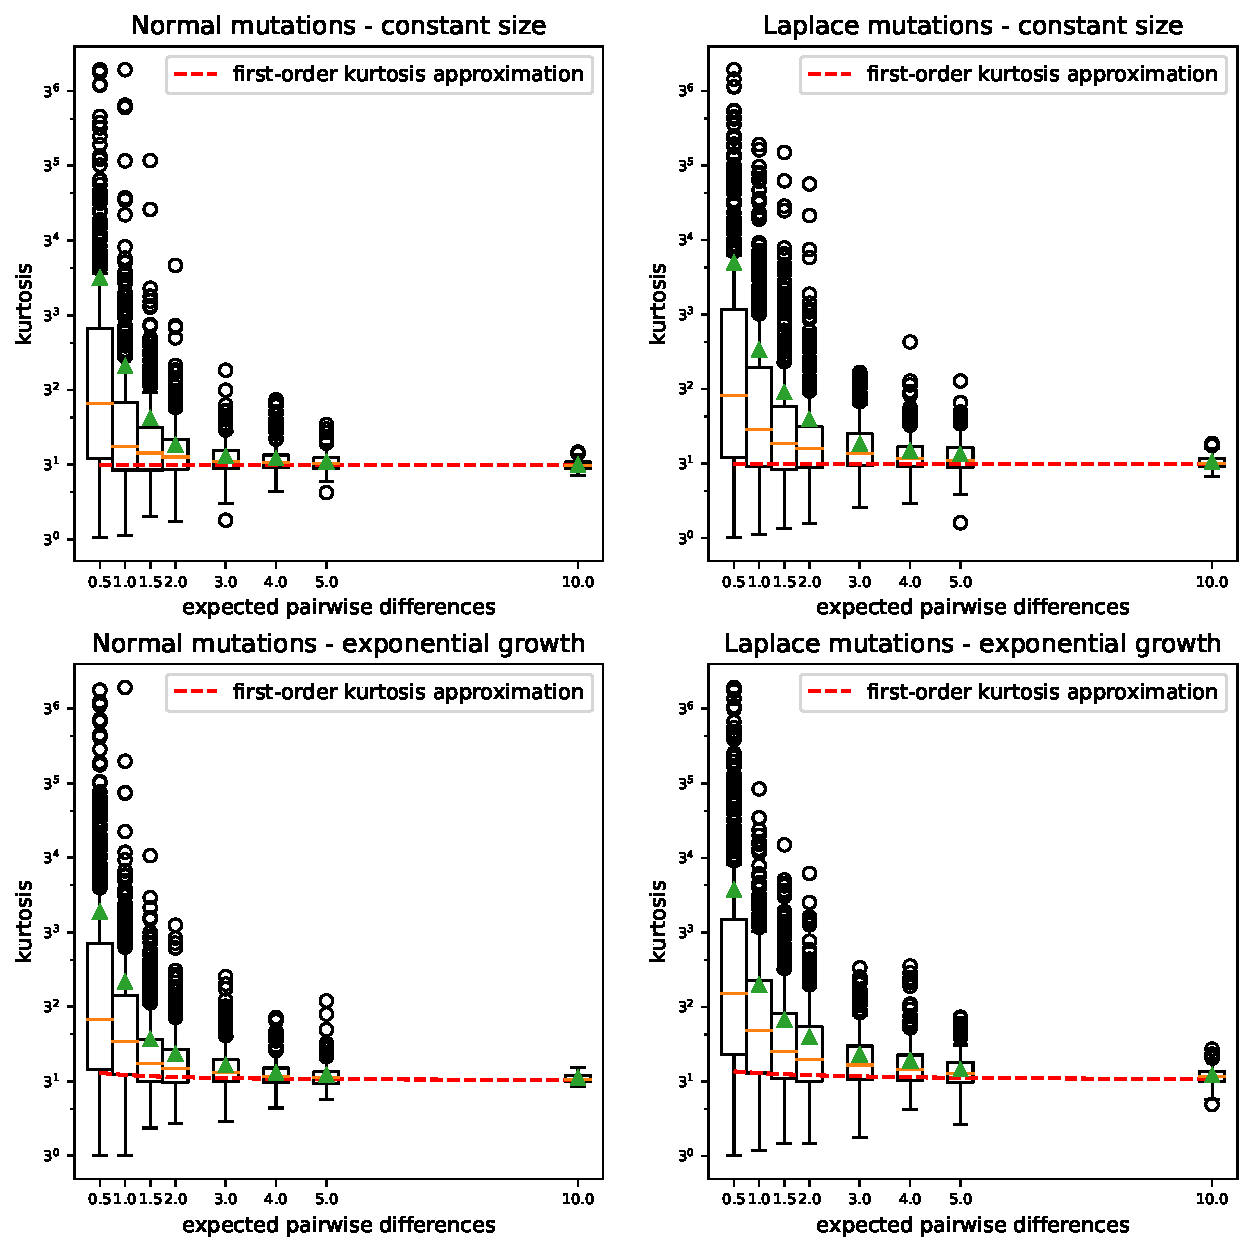
\includegraphics[width=\textwidth]{figures/kurt_sim.pdf}
  \captionof{figure}{\small The distribution of the population kurtosis under
    different levels of sparsity, mutational kernels, and demographies. The
    sparsity is varied by changing the expected number of pairwise differences
    at sites affecting the trait. Normal and Laplace distributions of mutational
    effects are compared. A constant size population is compared to an
    exponential growth scenario with growth rate equal to the reciprocal of the
    final effective population size. Green triangles denote the mean kurtosis.
    The dashed red lines give the first order approximation to the expected
    kurtosis given in equation \ref{eq:firstord}.}
  \label{fig:kurtsim}
\end{center}
Entire populations were simulated using msprime \citep{Kelleher2015} and
mutations were assigned effects from a zero-centered normal or Laplace
distribution. The effective population size and mutation rate were kept constant
and the expected number of pairwise difference was increased by increasing the
number of loci affecting the trait.

A first order approximation to the kurtosis is
\begin{equation}
    \label{eq:firstord} 
\kappa_Y^{(1)} = 3 + \frac{m_4/m_2^2 \frac{\CCC}{\E[\mathbbm{T}_{2,2}]}} {L \T \E[\mathbbm{T}_{2,2}]
    + m_4/m_2^2 \frac{\BBB}{\E[\mathbbm{T}_{2,2}]}}.
\end{equation}
Although this expression suggests that the expected $\kappa_Y$ will be greater
than under normality when external branches are longer ($\E[\mathbbm{T}_{4,4}] >
\frac{1}{6}\E[\mathbbm{T}_{3,4}] + \frac{1}{9}\E[\mathbbm{T}_{2,4}]$) and less
than under normality when they are longer ($\E[\mathbbm{T}_{4,4}] <
\frac{1}{6}\E[\mathbbm{T}_{3,4}] + \frac{1}{9}\E[\mathbbm{T}_{2,4}]$),
simulations show that the approximation is actually quite poor (Figure
\ref{fig:kurtsim}).
%%% Local Variables:
%%% TeX-master: "short_report.tex"
%%% End:

\section{Central moment derivations}
\label{moments}
We can use the low mutation rate approximation to the moment generating function
to calculate moments of the distribution of trait vales. We'll start by
calculating the first and second moments. We start, as we did in deriving the
normal distribution, by substituting the Taylor series of the mutational mgf.
\begin{equation}
  \label{eq:mgf_approx_sub}
  \varphi_{\mathbf{Y}}(\mathbf{k}) \approx \left[ 1 + \sum_{\omega \in \Omega}
    \E[T_\omega] \T \left( m_1 \sum_{a \in \omega} k_a +
    \frac{m_2}{2!}\left( \sum_{a \in \omega} k_a\right)^2 +
    \frac{m_3}{3!}\left( \sum_{a \in \omega} k_a\right)^3 +
    \frac{m_4}{4!}\left( \sum_{a \in \omega} k_a\right)^4 \ldots \right) \right]^L
\end{equation}
We can expand this out using multinomial coefficients to get
\begin{align}
  \label{eq:mgf_approx_expand}
  \varphi_{\mathbf{Y}}(\mathbf{k}) &\approx 1 +
  L\T \sum_{\omega \in \mathcal{O}} \E[T_{\omega}]\left( m_1 \sum_{a \in \omega} k_a +
  \frac{m_2}{2}\left( \sum_{a \in \omega} k_a\right)^2 + \ldots \right) \nonumber \\
  &+ \frac{L(L-1)}{2} \left(\T\right)^2 \sum_{\omega \in \Omega} E[T_{\omega}]^2
  \left( m_1 \sum_{a \in \omega} k_a +
  \frac{m_2}{2}\left( \sum_{a \in \omega} k_a\right)^2 + \ldots \right)^2 \nonumber \\
  &+ L(L-1)\left(\T\right)^2\sum_{\omega_1, \omega_2 \in \Omega}\E[T_{\omega_1}]\E[T_{\omega_2}]
  \left( m_1 \sum_{a \in \omega_1} k_a + \ldots \right)
  \left( m_1 \sum_{a \in \omega_2} k_a + \ldots \right) + \ldots.
\end{align}
The first coefficient is $\binom{L}{L-1,1,\mathbf{0}}$, the second is
$\binom{L}{L-2,2,\mathbf{0}}$, and the third is $\binom{L}{L-2,1,1,\mathbf{0}}$.
To calculate the moments of this distribution one takes the partial derivatives
of the mgf and sets the dummy variables to zero.
\begin{equation}
  \label{eq:deriv}
  \E[Y_1^{r_1}\ldots Y_n^{r_n}] = \frac{\partial^{r_1 + \ldots + r_n}}{\partial k_1^{r_1} \ldots \partial k_n^{r_n}}
  \varphi_{\mathbf{Y}}(\mathbf{k})\Bigr|_{\mathbf{k}=0}
\end{equation}
Using this to calculate the first moment of the trait distribution we get
\begin{equation}
  \label{eq:mom1}
  \E[Y_a] \approx L\T m_1 \sum_{\omega \in \Omega_a} \E[T_\omega].
\end{equation}
The second moment is more complicated because there are $k_a^2$ terms in all
three lines of equation \ref{eq:mgf_approx_expand}.
\begin{align}
  \E[Y_a^2] &\approx L\T m_2 \sum_{\omega \in \Omega_a} E[t_\omega] \nonumber \\
  &+ \frac{L(L-1)}{2} \left(\T \right)^2 m_1^2 \sum_{\omega \in \Omega_a} 2 \E[T_\omega]^2 \nonumber \\
  &+ L(L-1) \left(\T \right)^2 m_1^2 \sum_{\omega_1 , \omega_2 \in \Omega_{a+b}} 2 \E[T_{\omega_1}]E[T_{\omega_2}]
\end{align}
Terms with $(\T)^2$ are kept because they also include a second order term of
$L$ in front of them. We can now calculated the variance using $\Var[Y]=\E[Y^2] -
\E[Y]^2$. The squared first moment can be written as
\begin{align}
  \left(L\T m_1 \sum_{\omega \in \Omega_a} \E[t_\omega] \right)^2 &=
  L^2\left(\T\right)^2 m_1^2 \sum_{\omega \in \Omega_a} \E[T_\omega]^2 \nonumber \\
  &+ L^2\left(\T\right)^2 m_1^2 \sum_{\omega_1 , \omega_2 \in \Omega_{a+b}} \E[T_{\omega_1}]\E[T_{\omega_2}].
\end{align}
Subtracting this from the second moment gives
\begin{align}
  \label{eq:var}
  \Var[Y_a] &\approx L\T m_2 \sum_{\omega \in \Omega_a} \E[T_\omega] \nonumber \\
  &- L \left(\T\right)^2 m_1^2 \sum_{\omega \in \Omega_a}\E[T_\omega]^2 \nonumber \\
  &-  2L \left(\T\right)^2 m_1^2 \sum_{\omega_1 , \omega_2 \in \Omega_{a+b}} \E[T_{\omega_1}]\E[T_{\omega_2}] \nonumber \\
  &= L\T m_2 \sum_{\omega \in \Omega_a} \E[T_\omega] -
  L\left( \T m_1 \sum_{\omega \in \Omega_a} \E[T_\omega] \right)^2 \nonumber \\
  &= L\T m_2 \E[T_{MRCA}] - L\left( \T m_1 \E[T_{MRCA}] \right)^2  \\
  &\approx L\T m_2 \E[T_{MRCA}].  \nonumber
\end{align}

Due to the large number of terms I only derive the fourth moment of the trait
value distribution for the case when the mean mutational effect is zero. The
terms of \eqref{eq:mgf_approx_sub} appearing in the fourth moment after we apply
\eqref{eq:deriv} are
\begin{equation*}
  L \left(\T\right) \frac{m_4}{24}
  \sum_{\omega \in \Omega_a} \E[T_\omega] \left(\sum_{a \in \omega} k_a\right)^4
\end{equation*}
for the fourth moment along one branch,
\begin{equation*}
  \binom{L}{L-2,2,\mathbf{0}}\left(\T\right)^2\left(\frac{m_2}{2}\right)^2
  24 \sum_{\omega \in \Omega_a} \E[T_\omega]^2 \left(\sum_{a \in \omega} k_a\right)^4
\end{equation*}
for the second moment of the same branch chosen twice, and
\begin{equation*}
  \binom{L}{L-2,1,1,\mathbf{0}}\left(\T\right)^2\left(\frac{m_2}{2}\right)^2
  24 \sum_{\omega_1 , \omega_2 \in \Omega_{a+b}} \E[T_{\omega_1}]\E[T_{\omega_2}]
  \left(\sum_{a \in \omega_1} k_a\right)^2\left(\sum_{a \in \omega_2} k_a\right)^2
\end{equation*}
for the second moments on two different branches. Taking the fourth derivatives
of these in terms of the desired branch we get
\begin{align}
  \label{eq:mom4}
  \E[Y_a^4] &= L\T m_4 \E[T_{MRCA}] \nonumber \\
  &+ \frac{L(L-1)}{2} \left(\T\right)^2\left( \frac{m_2}{2} \right)^2
  24 \sum_{\omega \in \Omega_a} \E[t_\omega]^2 \nonumber \\
  &+ L(L-1) \left(\T\right)^2\left( \frac{m_2}{2} \right)^2
  24 \sum_{\omega_1 , \omega_2 \in \Omega_{a+b}} \E[T_{\omega_1}]\E[T_{\omega_2}] \nonumber \\
  &= L\T m_4 \E[T_{MRCA}] +
  3L(L-1)\left( \T m_2 \sum_{\omega \in \Omega_a} \E[T_\omega] \right)^2x \nonumber \\
  &= L\T m_4 \E[T_{MRCA}] +
  3L(L-1)\left( \T m_2 \E[T_{MRCA}] \right)^2 \\
  &\approx L\T m_4 \E[T_{MRCA}] +
  3\left(L \T m_2 \E[T_{MRCA}] \right)^2. \nonumber 
\end{align}

The kurtosis is defined as
\begin{equation*}
  Kurt[X]=\frac{E[(X-E[X])^4]}{E[(X-E[X])]^2]^2.}
\end{equation*}
This is the fourth central moment divided by the variance. It is possible to
calculate the kurtosis of a single trait value over evolutionary realization.
For ease of calculation, we'll examine this in the case where the mean mutation
effect (and therefore trait value) is zero. If we plug \eqref{eq:var} and
\eqref{eq:mom4} into the expression for the kurtosis we get
\begin{align*}
  \Kurt[Y_a] &= \frac{L\T m_4 \E[T_{MRCA}]}{\left(L\T m_2 \E[T_{MRCA}]\right)^2} +
  \frac{3L(L-1)\left( \T m_2  \E[T_{MRCA}]\right)^2}{\left(L\T m_2 \E[T_{MRCA}]\right)^2} \nonumber \\
  &= \frac{m_4}{L\T m_2^2\E[T_{MRCA}]} + \frac{3(L^2-L)}{L^2} \nonumber \\
  &= \frac{\kappa}{L\T \E[T_{MRCA}]} + 3\left( 1 - \frac{1}{L} \right).
\end{align*}

We also calculate some additional moments having less clear interpretations but
are useful later on when calculating the expected fourth central moment in the
population. The first of these is $\E[Y_a^3Y_b]$. The terms of
\eqref{eq:mgf_approx_sub} appearing in this are
\begin{equation*}
  L \left(\T\right) \frac{m_4}{24} 4 k_a^3k_b \sum_{\omega \in \Omega_{a+b}} \E[T_\omega]
\end{equation*}
and
\begin{equation*}
  L(L-1)\left(\T \frac{m_2}{2}\right)^2 k_a^2 \times 2k_ak_b
  \left( \sum_{\omega \in \Omega_{a+b}} \E[T_\omega] \right) \left( \sum_{\omega \in \Omega_a} \E[T_\omega] \right).
\end{equation*}
This ultimately gives
\begin{equation}
  \label{eq:m31}
  E[Y_a^3Y_b] = L \T m_4 \E[\tau_{a+b}] + 3L(L-1) \left(\T m_2\right)^2 \E[T_{MRCA}]\E[\tau_{a+b}].
\end{equation}
The next fourth moment of interest is $\E[Y_a^2Y_bY_c]$. The terms of
\eqref{eq:mgf_approx_sub} are
\begin{equation*}
  L \T \frac{m_4}{24} 12k_a^2k_bk_c \sum_{\omega \in \Omega_{a+b+c}} \E[T_\omega],
\end{equation*}
\begin{equation*}
  L(L-1) \left(\T \frac{m_2}{2}\right)^2 k_a^2 \times 2k_bk_c
  \left( \sum_{\omega \in \Omega_a} \E[T_\omega] \right)\left( \sum_{\omega \in \Omega_{a+b}} \E[T_\omega] \right),
\end{equation*}
and 
\begin{equation*}
  L(L-1) \left(\T \frac{m_2}{2}\right)^2 2k_ak_b \times 2k_ak_c \left( \sum_{\omega \in \Omega_{a+b}} \E[T_\omega] \right)
  \left( \sum_{\omega \in \omega_{b+c}} \E[T_\omega] \right).
\end{equation*}
Taking the appropriate derivatives of these gives
\begin{equation}
  \label{eq:m211}
  L \T m_4 \E[\tau_{a+b+c}] + L(L-1)\left(\T m_2\right)^2\E[T_{MRCA}]\E[\tau_{b+c}] +
  2L(L-1) \left(\T m_2\right)^2\E[\tau_{a+b}]\E[\tau_{a+c}].
\end{equation}
Individuals in the population are exchangeable as long as it is not structured.
The pairwise expected shared branch lengths are in that case all equal and we
can write \eqref{eq:m211} as
\begin{equation}
  \label{eq:m211s}
  L \T m_4 \E[\tau_{a+b+c}] + L(L-1)\left(\T m_2\right)^2\E[T_{MRCA}]\E[\tau_{a+b}] +
  2L(L-1) \left(\T m_2\right)^2\E[\tau_{a+b}]^2.
\end{equation}
The final moment we'll look at is $\E[Y_aY_bY_cY_d]$ which has relevant terms
%% The set of branches containing all individuals
\begin{equation*}
  L \T \frac{m_4}{24} 24k_ak_bk_ck_d \sum_{\omega \in \Omega_{a+b+c+d}} \E[T_\omega],
\end{equation*}
%% Cross set of a-b branches and c-d branches
\begin{equation*}
  L(L-1) \left(\T \frac{m_2}{2}\right)^2 2k_ak_b \times 2k_ck_d \left( \sum_{\omega \in \Omega_{a+b}} \E[T_\omega] \right)
  \left( \sum_{\omega \in \Omega_{c+d}} \E[T_\omega] \right),
\end{equation*}
%% Cross set of a-c branches and b-d branches
\begin{equation*}
  L(L-1) \left(\T \frac{m_2}{2}\right)^2 2k_ak_c \times 2k_bk_d \left( \sum_{\omega \in \Omega_{a+c}} \E[T_\omega] \right)
  \left( \sum_{\omega \in \Omega_{b+d}} \E[T_\omega] \right),
\end{equation*}
and
%% cross set of a-d branches and b-c branches
\begin{equation*}
  L(L-1) \left(\T \frac{m_2}{2}\right)^2 2k_ak_d \times 2k_bk_c \left( \sum_{\omega \in \Omega_{a+d}} \E[T_\omega] \right)
  \left( \sum_{\omega \in \omega_{b+c}} \E[T_\omega] \right).
\end{equation*}
When the appropriate fourth order partial derivatives are taken of this we get
\begin{align*}
  L \T m_4 \E[\tau_{a+b+c+d}] \\
  + L(L-1)\left(\T m_2\right)^2\E[\tau_{a+b}]\E[\tau_{c+d}] \\
  + L(L-1)\left(\T m_2\right)^2\E[\tau_{a+c}]\E[\tau_{b+d}] \\
  + L(L-1)\left(\T m_2\right)^2\E[\tau_{a+d}]\E[\tau_{b+c}].
\end{align*}
We can again simplify this expression for populations with exchangeable
individuals. This gives
\begin{equation}
  \label{eq:m1111}
  L \T m_4 \E[\tau_{a+b+c+d}] + 3L(L-1)\left(\T m_2\right)^2\E[\tau_{a+b}]^2.
\end{equation}

The expected kurtosis in the population is a quotient and therefore annoying to
calculate. Instead we will calculate the expected fourth central moment. 
\begin{equation}
  \E[M_{4,Y}] = \E\left[\frac{1}{N} \sum \left( Y_i - \frac{\sum Y_j}{N} \right)^4 \right].
\end{equation}
Examining the sum inside the expectation we see that 
\begin{align}
  \label{eq:expandkurt}
  \E\left[ \left( Y_i - \frac{\sum Y_j}{N} \right)^4 \right] &= \E[Y_i^4] - 
                                                              4\E\left[ Y_i^3 \frac{\sum Y_j}{N} \right] + 
                                                              6\E\left[Y_i^2\left(\frac{\sum Y_j}{N}\right)^2\right] - 
                                                              4\E\left[Y_i\left(\frac{\sum Y_j}{N}\right)^3\right]+ 
                                                              \left(\frac{\sum Y_j}{N}\right)^4 \nonumber \\
                                                            &= \E[Y_i^4] - 
                                                              \frac{4}{N}\sum_j \E[Y_i^3Y_j] + 
                                                              \frac{6}{N^2}\sum_{j,k} \E[Y_i^2Y_jY_k] \nonumber\\
                                                              &-\frac{4}{N^3}\sum_{j,k,l}\E[Y_iY_jY_kY_l] + 
                                                              \frac{1}{n^4}\sum_{j,k,l,d}\E[Y_jY_kY_lY_d].
\end{align}
In calculating these expectations we have to remember that the value depends
only on the number of times each variable appears in the expectation. That is,
$\E[Y_1^2Y_2Y_3]$ is equivalent to $\E[Y_1Y_2^3Y_3]$ as long as all individuals
in the population are exchangeable. The resulting expansion of
\eqref{eq:expandkurt} is therefore quite ugly. It can be simplified by only
considering terms of order one. Other terms can be ignored since we are assuming
there are a large number of individuals in the population. This yields
\begin{align}
  \label{eq:popkurt}
  \E\left[ \left( Y_i - \frac{\sum Y_j}{N} \right)^4 \right] &=
  \E[Y_i^4]  - \frac{4(n-1)}{n}\E[Y_i^3Y_j] + \frac{6(n-1)(n-2)}{n^2}\E[Y_i^3Y_jY_k]  \nonumber \\
  &- \frac{4(n-1)(n-2)(n-3)}{n^3}\E[Y_iY_jY_kY_l] \nonumber \\
  &+ \frac{(n-1)(n-2)(n-3)(n-4)}{n^4}\E[Y_jY_kY_lY_d]
  + O(n^{-1}) \nonumber \\
  &\approx \E[Y_i^4]  - 4\E[Y_i^3Y_j] + 6\E[Y_i^2Y_jY_k] - 3\E[Y_iY_jY_kY_l].
\end{align}

The first term, $\E[Y_i^4]$ was derived in equation \eqref{eq:mom4} as
\begin{equation*}
  L\T m_4 \E[T_{MRCA}] + 3L(L-1)\left( \T m_2 \E[T_{MRCA}] \right)^2.
\end{equation*}
The second term, $\E[Y_i^3Y_j]$ was derived in equation \eqref{eq:m31} as
\begin{equation*}
  L \T m_4 \E[\tau_{a+b}] + 3L(L-1) \left(\T m_2\right)^2 \E[T_{MRCA}]\\E[\tau_{a+b}].
\end{equation*}
The third term, $\E[Y_i^2Y_jY_k]$ was derived in equation \eqref{eq:m211} as
\begin{equation*}
  L \T m_4 \E[\tau_{a+b+c}] + L(L-1)\left(\T m_2\right)^2\E[T_{MRCA}]\E[\tau_{a+b}] +
  2L(L-1) \left(\T m_2\right)^2\E[\tau_{a+b}]^2.
\end{equation*}
The fourth term, $\E[Y_iY_jY_kY_l]$ was derived in equation \eqref{eq:m1111} as
\begin{equation*}
  L \T m_4 \E[\tau_{a+b+c+d}] + 3L(L-1)\left(\T m_2\right)^2\E[\tau_{a+b}]^2.
\end{equation*}
Plugging these into \eqref{eq:popkurt} we get
\begin{align}
  \label{eq:popm4coal}
  \E[M_{4,Y}] &\approx L \T m_4 \left( \E[T_{MRCA}] - 4\E[\tau_{a+b}] + 6\E[\tau_{a+b+c}] -3\E[\tau_{a+b+c+d}] \right)\nonumber \\
  &+ 3\left( L \T m_2 \right)^2\left(\E[T_{MRCA}]- \E[\tau_{a+b}]\right)^2.
\end{align}
With some simple manipulation this can be rewritten in terms of $\mathbbm{T}_{i,j}$.

% These expressions approximate $L(L-1)$ as $L^2$ as part of the low mutation rate
% approximation. The fourth central moment of a normal distribution is
% $3\sigma^4$. Using the expected population  variance we get $3\left(L\T m_2
% \E[T_{MRCA}]- \E[\tau_{a+b}]\right)^2$. It is clear from \eqref{eq:popm4coal} that
% as $L\T$ gets large the second term will dominate and the population will have
% the same expected kurtosis as a normal distribution. The expected population kurtosis
% is
% \begin{equation*}
%   \E[\mbox{Kurt}] \approx 3 + \frac{\kappa( \E[T_{MRCA}] - 4\E[\tau_{a+b}] +
%     6\E[\tau_{a+b+c}] -3\E[\tau_{a+b+c+d}])}{L \T \E[T_{MRCA}]- \E[\tau_{a+b}]}.
% \end{equation*}
% This expression can be written in an easier to interpret form by noting that
% $\E[\tau_{a+b}]=\E[T_{MRCA}] - \E[T_2]$, $\E[\tau_{a+b+c}]=\E[T_{MRCA}] - \E[T_3]$,
% $\E[\tau_{a+b+c+d}]=\E[T_{MRCA}] - \E[T_4]$, where $T_i$ is the expected time it
% takes for $i$ lineages to coalesce.
% \begin{equation}
%   \label{eq:popkurtcoal}
%   \E[\mbox{Kurt}] \approx 3 + \frac{\kappa( 4T_2 - 6T_3 + 3T_4)}{L \T T_2}.
% \end{equation}
% In a constant size population this would be $3 + \frac{\kappa}{2L\T}$.

%%% Local Variables:
%%% TeX-master: "short_report.tex"
%%% End:

\end{document}


